\chapter{Motors d'Inducció Trifàsics}\label{sec:motors-ind}\index{motors d'inducció}

\section{Introducció}

Es tracten en aquest capítol els motors d'inducció trifàsics.

Es farà primer una petita introducció a les unitats de mesura anglesa relacionades amb els motors, ja que és molt freqüent trobar-se amb aquestes unitats en llibres, articles tècnics i catàlegs.

Quan es tracte amb motors elèctrics cal anar amb compte entre les magnituds elèctriques i les mecàniques; un motor, per exemple, absorbeix una potència elèctrica de la xarxa per funcionar, i proporciona una potència mecànica en el seu eix. Per tal de distingir aquests dos tipus de magnituds s'utilitzarà el subíndex «m» en les magnituds mecàniques.

\section{Unitats de mesura angleses}\index{unitats de mesura angleses}

\subsection{Unitats base}\index{unitats de mesura angleses!unitats base}

En la taula \vref{taula:angleses-base} es poden veure les unitats base angleses que són d'aplicació en l'àmbit dels motors elèctrics:
\begin{longtable}[h]{llc}
   \caption{\label{taula:angleses-base}Unitats base}\\
   \toprule[1pt]
    Magnitud & Unitat & Símbol \\
   \midrule
   \endfirsthead
   \caption[]{Unitats base (\emph{ve de la pàgina anterior})}\\
   \toprule[1pt]
    Magnitud & Unitat & Símbol \\
   \midrule
   \endhead
   \midrule
   \multicolumn{3}{r}{\sffamily\bfseries\color{NavyBlue}(\emph{continua a la pàgina següent})}
   \endfoot
   \endlastfoot
   longitud & peu & ft \\
   massa & «slug» & slug \\
   temps & segon & s\\
   força & lliura-força & lbf \\
   \bottomrule[1pt]
\end{longtable}
\index{peu}\index{segon}\index{lliure}\index{lliura-força}\index{slug}\index{ft}\index{s}\index{lbf}\index{s}

La relació entre aquestes quatre unitats base és la següent:
\begin{equation}
    \SI{1}{lbf} \equiv \SI{1}{slug.ft.s^{-2}}
\end{equation}

\subsection{Altres unitats}\index{unitats de mesura angleses!altres unitats}

En la taula \vref{taula:altres-angleses} es poden veure altres unitats que també són d'aplicació en l'àmbit dels motors elèctrics; totes pertanyen al sistema d'unitats angleses, tret del cavall vapor:
\begin{longtable}[h]{llc}
   \caption{\label{taula:altres-angleses}Altres unitats}\\
   \toprule[1pt]
    Magnitud & Unitat & Símbol \\
   \midrule
   \endfirsthead
   \caption[]{Altres unitats (\emph{ve de la pàgina anterior})}\\
   \toprule[1pt]
    Magnitud & Unitat & Símbol \\
   \midrule
   \endhead
   \midrule
   \multicolumn{3}{r}{\sffamily\bfseries\color{NavyBlue}(\emph{continua a la pàgina següent})}
   \endfoot
   \endlastfoot
   longitud & polsada & in \\
   massa & lliura «avoirdupois» & lb \\
   potència & «horsepower» & HP \\
   potència & «horsepower» mètric & \si{HPm} \\
   potència & «horsepower» elèctric & \si{HPe} \\
   potència & cavall vapor & CV \\
   \bottomrule[1pt]
\end{longtable}
\index{lliura «avoirdupois»}\index{lb}\index{horsepower}\index{HP}\index{horsepower mètric}\index{HPm}
\index{horsepower elèctric}\index{HPe}\index{cavall vapor}\index{CV}


\subsection{Factors de conversió}\index{unitats de mesura angleses!factors de conversió}

Es donen en aquesta secció factors de conversió entre unitats angleses i les seves unitats equivalents del sistema internacional d'unitats (SI).\footnote{Aneu a l'apèndix \ref{sec:SI} per veure una explicació completa del sistema internacional d'unitats (SI).}

Els factors de conversió que es poden veure a continuació, són els recomanats pel NIST «National Institute of Standards and Technology».\footnote{Aneu a l'apèndix \ref{sec:SI} i vegeu la secció \ref{sec:SI-fact-conv} per a més informació.}

\begin{itemize}
    \item \textbf{Longitud}. Els factors de conversió del peu i de la polsada, són:
    \begin{subequations}
    \begin{alignat}{3}
      \SI{1}{ft} &= \SI{0,3048}{m} &&\quad(\text{valor exacte}) \\
      \SI{1}{in} &= \SI{2,54}{cm} &&\quad(\text{valor exacte})
    \end{alignat}
    \end{subequations}

    El peu és un múltiple  de la polsada:
    \begin{equation}
      \SI{1}{ft} = \SI{12}{in}\quad(\text{valor exacte})
    \end{equation}

    \item \textbf{Massa}. Els factors de conversió de l'«slug»  i de la lliura «avoirdupois», són:
    \begin{subequations}
    \begin{align}
      \SI{1}{slug} &= \SI{14,59390}{kg} \\
      \SI{1}{lb} &= \SI{0,45359237}{kg}\quad(\text{valor exacte})
    \end{align}
    \end{subequations}

    La relació entre l'«slug» i la lliura «avoirdupois» és un valor adimensional:
    \begin{equation}
        \frac{\SI{1}{slug}}{\SI{1}{lb}}=\num{32,17404}
    \end{equation}

    Aquest valor és igual al valor de l'acceleració de la gravetat estàndard, quan s'expressa en \si{ft/s^2}.

    \item \textbf{Força}. El factor de conversió de la lliura-força, és:
    \begin{equation}
        \SI{1}{lbf} = \SI{4,448222}{N}
    \end{equation}

    \item \textbf{Parell}. Els factors de conversió de la lliura-força peu  i de la lliura-força polsada, són:
    \begin{subequations}
    \begin{align}
      \SI{1}{lbf.ft} &= \SI{1,355818}{N.m} \\
      \SI{1}{lbf.in} &= \SI{0,1129848}{N.m}
    \end{align}
    \end{subequations}

    \item \textbf{Moment d'inèrcia}. Els factors de conversió de l'«slug» peu quadrat, de la lliura «avoirdupois» peu quadrat   i de la lliura «avoirdupois» polsada quadrada, són:
    \begin{subequations}
    \begin{align}
        \SI{1}{slug.ft^2} &= \SI{1,355818}{kg.m^2} \\
        \SI{1}{lb.ft^2} &= \SI{4,214011e-2}{kg.m^2} \\
        \SI{1}{lb.in^2} &= \SI{2,926397e-4}{kg.m^2}
    \end{align}
    \end{subequations}

    \item \textbf{Potència mecànica}. Els factors de conversió de la lliura-força peu per segon, del «horsepower»,  del «horsepower» mètric i del cavall vapor, són:
    \begin{subequations}
    \begin{align}
      \SI{1}{lbf.ft/s} &= \SI{1,355818}{W} \\
      \SI{1}{HP} &= \SI{745,6999}{W} \\
      \SI{1}{HPm} &= \SI{735,4988}{W} \\
      \SI{1}{CV} &= \SI{735,4988}{W}
    \end{align}
    \end{subequations}

    El «horsepower» és un múltiple  de la lliura-força peu per segon. El «horsepower» mètric i el cavall vapor són unitats equivalents:
    \begin{subequations}
    \begin{alignat}{3}
      \SI{1}{HP} &= \SI{550}{lbf.ft/s}  &&\quad(\text{valor exacte}) \\
      \SI{1}{CV} &= \SI{1}{HPm} &&\quad(\text{valor exacte})
    \end{alignat}
    \end{subequations}


    \item \textbf{Potència elèctrica}. El factor de conversió del
    «horsepower» elèctric, és:
    \begin{equation}
        \SI{1}{HPe} = \SI{746}{W}\quad(\text{valor exacte})
    \end{equation}
  \end{itemize}


\section{Equacions bàsiques}\index{motors d'inducció!equacions bàsiques}

Es relaciona a continuació una sèrie de variables elèctriques i mecàniques utilitzades normalment per descriure el comportament dels motors elèctrics:

\begin{list}{}
   {\setlength{\labelwidth}{12mm} \setlength{\leftmargin}{12mm} \setlength{\labelsep}{2mm}}
   \item[$\boldsymbol{\theta\ped{m}}$] Angle de rotació mecànic, expressat en \si{rad}.
   \item[$\boldsymbol{\omega\ped{m}}$] Velocitat de rotació mecànica, expressada en \si{rad/s}.
   \item[$\boldsymbol{n\ped{m}}$] Velocitat de rotació mecànica, expressada en \si{r/min}.\footnote{r és el símbol de «revolució»; aneu a l'apèndix \ref{sec:SI} i vegeu la secció \ref{sec:unit-maq-rotativ} per a més informació.}
   \item[$\boldsymbol{\theta}$] Angle de rotació elèctric, expressat en \si{rad}.
   \item[$\boldsymbol{\omega}$] Velocitat de rotació elèctrica, expressada en \si{rad/s}.
   \item[$\boldsymbol{n}$] Velocitat de rotació elèctrica, expressada en \si{r/min}.
   \item[$\boldsymbol{f}$] Freqüència elèctrica de l'estator, expressada en \si{Hz}. Els valors usuals són \SI{50}{Hz} i \SI{60}{Hz}.
   \item[$\boldsymbol{p}$] Nombre de pols del motor.\footnote{El nombre de pols $p$  és sempre un nombre parell (2, 4, 6, ...), això fa que en alguns llibres i articles tècnics es defineixi $p$ com el nombre de parells de pols del motor       (1, 2, 3, ...).}
   \item[$\boldsymbol{s}$] Lliscament, adimensional.
   \item[$\boldsymbol{T\ped{m}}$] Parell mecànic proporcionat per l'eix del motor, expressat en \si{N.m} (altres unitats equivalents: \si{lbf.ft}, \si{lbf.in}).
   \item[$\boldsymbol{T\ped{load}}$] Parell mecànic resistent que ofereix una càrrega (ventilador, bomba, etc.) en ser arrossegada per un motor, expressat en \si{N.m} (altres unitats equivalents: \si{lbf.ft}, \si{lbf.in}).
   \item[$\boldsymbol{J}$] Moment d'inèrcia, expressat en \si{kg.m^2} (altres unitats equivalents: \si{slug.ft^2}, \si{lb.ft^2}, \si{in.ft^2}).
   \item[$\boldsymbol{H}$] Constant d'inèrcia, expressada en \si{s} (o de forma més explícita:
   $\si{s.rad^2.W/VA} \equiv \si{rad^2.J/VA}$).
   \item[$\boldsymbol{P\ped{m}}$] Potència mecànica, expressada en \si{W} (altres unitats equivalents: \si{lbf.ft/s}, \si{HP},  \si{HPm}, \si{CV}).
   \item[$\boldsymbol{P}$] Potència elèctrica activa, expressada en \si{W} (altres unitats equivalents: \si{HPe}).
   \item[$\boldsymbol{S}$] Potència elèctrica aparent, expressada en \si{VA}.
   \item[$\boldsymbol{\eta}$] Rendiment, adimensional.
   \item[$\boldsymbol{U}$] Tensió fase--fase aplicada al motor, expressada en \si{V}.
   \item[$\boldsymbol{I}$] Corrent de fase absorbit pel motor, expressat en \si{A}.
   \item[$\boldsymbol{\cos\varphiup}$] Factor de potència, on $\varphiup$ és l'angle entre el fasor de la tensió fase--neutre aplicada al motor i el fasor del corrent de fase absorbit pel motor.
\end{list}

La relació entre les variables mecàniques i les elèctriques ve donada pel nombre de pols $p$ del motor:
\begin{equation}\label{eq:vel-ele-mec}
    \theta\ped{m} = \frac{2\theta}{p} \qquad\qquad
    \omega\ped{m} = \frac{2\omega}{p} \qquad\qquad
    n\ped{m} = \frac{2n}{p}
\end{equation}

Per  convertir una velocitat de rotació expressada en \si{rad/s} en una velocitat de rotació expressada en \si{r/min}, cal fer la conversió:
\begin{equation}
 1\frac{\si{rad}}{\si{s}} \times \frac{\SI{60}{s}}{\SI{1}{min}} \times \frac{\SI{1}{r}}{2\piup\,\si{rad}} = \frac{30}{\piup}\frac{\si{r}}{\si{min}}
 \end{equation}

 Per tant, per passar de $\omega$ a $n$, o de $\omega\ped{m}$ a $n\ped{m}$, podem usar les equacions següents:
\begin{subequations}
\begin{align}
    n        &= \frac{30}{\piup} \,\omega \\[1ex]
    n\ped{m} &= \frac{30}{\piup} \,\omega\ped{m}
\end{align}
\end{subequations}

La velocitat nominal d'un motor d'inducció és sempre propera a l'anomenada velocitat síncrona, però sense arribar-hi, ja que en aquest cas el parell mecànic que subministraria el motor seria nul.

La velocitat síncrona elèctrica depèn de la freqüència elèctrica de la tensió que l'alimenta; la velocitat síncrona mecànica s'obté a partir de la velocitat síncrona elèctrica i de  les equacions \eqref{eq:vel-ele-mec}:
\begin{subequations}
\begin{align}
    \omega\ped{sinc} &= 2 \piup f & n\ped{sinc} &= 60 f \\[1ex]
    \omega\ped{m,sinc} &= \frac{4 \piup f}{p} & n\ped{m,sinc} &= \frac{120 f}{p}\label{eq:vel-mec-sinc}
\end{align}
\end{subequations}

El lliscament $s$ es defineix com el quocient de la diferència entre la velocitat síncrona d'un motor i la velocitat real, i la velocitat síncrona:
\begin{equation}\label{eq:lliscament}\index{lliscament}
    s = \frac{n\ped{m,sinc}-n\ped{m}}{n\ped{m,sinc}} =
    \frac{n\ped{sinc}-n}{n\ped{sinc}} =
    \frac{\omega\ped{m,sinc}-\omega\ped{m}}{\omega\ped{m,sinc}} =
    \frac{\omega\ped{sinc}-\omega}{\omega\ped{sinc}}
\end{equation}

D'aquestes relacions es dedueix que quan el motor està parat (velocitat nuŀla) el lliscament és: $s=1$, i que si el motor arribés a la velocitat síncrona el lliscament seria: $s=0$. A partir de les equacions anterior podem escriure la relació entre la velocitat de rotació i la velocitat síncrona:
\begin{align}
    \omega\ped{m} &= (1-s) \omega\ped{m,sinc} & n\ped{m} &= (1-s) n\ped{m,sinc} \label{eq:wm-wsinc}
\end{align}

\addcontentsxms{Nombre de pols i lliscament d'un motor}
\begin{exemple}[Nombre de pols i lliscament d'un motor]
    Sabent que la velocitat nominal d'un motor és: $n\ped{m,N} = \SI{1440}{r/min}$, quan es connecta a una xarxa elèctrica de: $f = \SI{50}{Hz}$,  es tracta de trobar el nombre de pols i el lliscament nominal del motor.

    A partir de l'equació \eqref{eq:vel-mec-sinc} donem diversos valors a $p$ i troben les velocitats $n\ped{m,sinc}$ corresponents:
    \begin{align*}
      p = 2 \quad  &\Rightarrow \quad n\ped{m,sinc} = \frac{120 \times \SI{50}{Hz}}{2} = \SI{3000}{r/min}\\[0.5ex]
      p = 4 \quad  &\Rightarrow \quad n\ped{m,sinc} = \frac{120 \times \SI{50}{Hz}}{4} = \SI{1500}{r/min}\\[0.5ex]
      p = 6 \quad  &\Rightarrow \quad n\ped{m,sinc} = \frac{120 \times \SI{50}{Hz}}{6} = \SI{1000}{r/min}
    \end{align*}

    Donat que sabem que la velocitat nominal d'un motor és propera a la velocitat síncrona, deduïm que aquest motor té 4 pols, i que la velocitat síncrona corresponent és \SI{1500}{r/min}.

    El lliscament nominal s'obté a partir de l'equació \eqref{eq:lliscament}:
    \[
      s\ped{N} = \frac{\SI{1500}{r/min} - \SI{1440}{r/min}}{\SI{1500}{r/min}} = \num{0,04}
    \]
\end{exemple}

El rendiment d'un motor ve donat pel quocient entre la potència mecànica subministrada i la potència activa elèctrica absorbida:
\begin{equation}\index{rendiment}\index{potència mecànica}
    \eta = \frac{P\ped{m}}{P}
\end{equation}

A partir de la relació elèctrica: $P = S \cos\varphiup$, tenim la següent relació entre la potència mecànica subministrada per un motor i la potència aparent elèctrica absorbida:
\begin{equation}
    S = \sqrt{3} U I = \frac{P\ped{m}}{\eta \cos\varphiup}
\end{equation}

Per  convertir una potència mecànica expressada en HP o en CV en una  potència mecànica expressada en kW, cal  fer les conversions:
\begin{subequations}
\begin{align}
  \SI{1}{HP} \times \frac{\SI{745,6999}{W}}{\SI{1}{HP}} \times \frac{\SI{1}{kW}}{\SI{1000}{W}} &= \SI{0,7456999}{kW} \\[1ex]
  \SI{1}{CV} \times \frac{\SI{735,4988}{W}}{\SI{1}{CV}} \times \frac{\SI{1}{kW}}{\SI{1000}{W}} &= \SI{0,7354988}{kW}
\end{align}
\end{subequations}

 A més, tenint en compte que quan dividim una potència activa elèctrica per $\cos\varphiup$, obtenim una potència a parent elèctrica, tenim les expressions següents entre $P\ped{m}$, expressada en HP o en CV, i $S$ expressada en kVA:
\begin{align}
    S/{\scriptstyle\si{kVA}} &= \frac{\num{0,7456999}}{\eta \cos\varphiup}\,   P\ped{m}/{\scriptstyle\si{HP}} \\[1ex]
    S/{\scriptstyle\si{kVA}} &= \frac{\num{0,7354988}}{\eta \cos\varphiup}\,   P\ped{m}/{\scriptstyle\si{CV}}
\end{align}

En el punt nominal de funcionament d'un motor, els valors del rendiment solen ser en general de l'ordre de 0,9 o superiors ($\eta\ped{N} \approx \num{0,9}$) i els valors del factor de potència solen ser de l'ordre de 0,85 o superiors ($\cos\varphiup\ped{N} \approx \num{0,85}$), això fa que els quocients $\num{0,7456999}/(\num{0,9} \times \num{0,85})$ o $\num{0,7354988}/(\num{0,9} \times \num{0,85})$ tinguin un valor aproximat a 1. Per tant, de forma aproximada es compleix que el valor de la potència nominal aparent absorbida pel motor, expressada en kVA, és igual al valor de la potència mecànica nominal subministrada pel motor, expressada en HP o en CV:
\begin{equation}\label{eq:kVA-CV-HP}
    S\ped{N}/{\scriptstyle \si{kVA}} \quad\approx\quad  P\ped{m,N}/{\scriptstyle \si{HP}} \quad\approx\quad  P\ped{m,N}/{\scriptstyle \si{CV}}
\end{equation}


El parell mecànic subministrat per un motor ve donat pel quocient entre la potència mecànica subministrada i la velocitat mecànica de rotació:
\begin{equation}\index{parell!mecànic}
    T\ped{m} = \frac{P\ped{m}}{\omega\ped{m}}\label{eq:T-P-w}
\end{equation}

Per  obtenir un  parell mecànic expressat en \si{N.m}, a partir d'una potència mecànica expressada en kW, en HP o en CV, i d'una velocitat de rotació expressada en \si{r/min}, cal  fer les conversions:
\begin{subequations}
\begin{align}
    \frac{\SI{1}{kW} \times \frac{\SI{1000}{W}}{\SI{1}{kW}}}{1\frac{\si{r}}{\si{min}} \times \frac{\SI{1}{min}}{\SI{60}{s}} \times \frac{2\piup\,\si{rad}}{\SI{1}{r}}} &=  \num{9549,2966}\, \frac{\si{W}}{\si{rad/s}} = \SI{9549,2966}{N.m} \\[1ex]
    \frac{\SI{1}{HP} \times \frac{\SI{745,6999}{W}}{\SI{1}{HP}}}{1\frac{\si{r}}{\si{min}} \times \frac{\SI{1}{min}}{\SI{60}{s}} \times \frac{2\piup\,\si{rad}}{\SI{1}{r}}} &=  \num{7120,9095}\, \frac{\si{W}}{\si{rad/s}} = \SI{7120,9095}{N.m} \\[1ex]
    \frac{\SI{1}{CV} \times \frac{\SI{735,4988}{W}}{\SI{1}{CV}}}{1\frac{\si{r}}{\si{min}} \times \frac{\SI{1}{min}}{\SI{60}{s}} \times \frac{2\piup\,\si{rad}}{\SI{1}{r}}} &=  \num{7023,4962}\, \frac{\si{W}}{\si{rad/s}} = \SI{7023,4962}{N.m}
\end{align}
\end{subequations}

Addicionalment, per  convertir aquests parells mecànics expressats en \si{N.m}, en parells mecànics expressats en \si{lbf.ft}, cal  fer les conversions:
\begin{subequations}
\begin{align}
    \SI{9549,2966}{N.m} \times \frac{\SI{1}{lbf}}{\SI{1,355818}{N.m}} &= \SI{7043,1994}{lbf.ft} \\[1ex]
    \SI{7120,9095}{N.m} \times \frac{\SI{1}{lbf}}{\SI{1,355818}{N.m}} &= \SI{5252,1131}{lbf.ft} \\[1ex]
    \SI{7023,4962}{N.m} \times \frac{\SI{1}{lbf}}{\SI{1,355818}{N.m}} &= \SI{5180,2647}{lbf.ft}
\end{align}
\end{subequations}

Per tant, per  obtenir $T\ped{m}$ expressat en \si{N.m} o en \si{lbf.ft}, a partir de $P\ped{m}$ expressada en kW, en HP o en CV, i $\omega\ped{m}$ expressada en \si{r/min} (o sigui $n\ped{m}$),  podem usar les equacions següents:
\begin{subequations}
\begin{align}
    T\ped{m}/{\scriptstyle \si{N.m}} &= \num{9549,30}\,  \frac{P\ped{m}/{\scriptstyle \si{kW}}}{n\ped{m}} \\[1ex]
    T\ped{m}/{\scriptstyle \si{N.m}} &= \num{7120,91}\,  \frac{P\ped{m}/{\scriptstyle \si{HP}}}{n\ped{m}}\label{eq:T-N-m} \\[1ex]
    T\ped{m}/{\scriptstyle \si{N.m}} &= \num{7023,50}\,  \frac{P\ped{m}/{\scriptstyle \si{CV}}}{n\ped{m}} \\[1ex]
    T\ped{m}/{\scriptstyle \si{lbf.ft}} &= \num{7043,20}\,  \frac{P\ped{m}/{\scriptstyle \si{kW}}}{n\ped{m}} \\[1ex]
    T\ped{m}/{\scriptstyle \si{lbf.ft}} &= \num{5252,11}\,  \frac{P\ped{m}/{\scriptstyle \si{HP}}}{n\ped{m}}\label{eq:T-lbf-ft} \\[1ex]
    T\ped{m}/{\scriptstyle \si{lbf.ft}} &= \num{5180,26}\,  \frac{P\ped{m}/{\scriptstyle \si{CV}}}{n\ped{m}}
\end{align}
\end{subequations}

\addcontentsxms{Parell nominal  d'un motor}
\begin{exemple}[Parell nominal  d'un motor]
    Sabent que la velocitat nominal d'un motor és: $n\ped{m,N} = \SI{1440}{r/min}$, i que la seva potència nominal és: $P\ped{m,N} = \SI{7,5}{HP}$,   es tracta de trobar el parell nominal del motor $T\ped{m,N}$ expressat en \si{N.m} i en \si{lbf.ft}.

    A partir de les equacions  \eqref{eq:T-N-m} i \eqref{eq:T-lbf-ft} tenim:
    \begin{align*}
      T\ped{m,N} &= \num{7120,91} \times \frac{\SI{7,5}{HP}}{\SI{1440}{r/min}} = \SI{37,09}{N.m} \\[1ex]
      T\ped{m,N} &= \num{5252,11} \times \frac{\SI{7,5}{HP}}{\SI{1440}{r/min}} = \SI{27,35}{lbf.ft}
    \end{align*}
\end{exemple}


El moment d'inèrcia total $J$ vist per un motor, és en general la suma del moment d'inèrcia del  motor mateix $J\ped{motor}$ més el moment d'inèrcia de la càrrega arrossegada pel motor $J\ped{load}$. En el cas que entre el motor i la càrrega hi hagi un sistema d'engranatges que faci que la càrrega giri a una velocitat diferent de la velocitat del motor, el  moment d'inèrcia total vist pel motor serà:
\begin{equation}\index{moment d'inèria}\index{J@$J$}
    J = J\ped{motor} +  J\ped{load}
    \left(\frac{n\ped{m,load}}{n\ped{m,motor}}\right)^2
\end{equation}

En alguns llibres, articles i catàlegs, sobretot en anglès, en lloc d'utilitzar el símbol $J$ per designar el moment d'inèrcia, s'utilitza el símbol equivalent $W\hspace{-0.2em}R^2$. El sentit de $W\hspace{-0.2em}R^2$ és clar si pensem que un moment d'inèrcia és el producte d'una massa o «pes» («weight» en anglès) per un radi de gir al quadrat.

La constant d'inèrcia $H$ es defineix com la relació entre l'energia cinètica de rotació del motor  a la velocitat nominal: $\frac{1}{2} J \omega\ped{m,N}^2$, i la  potència elèctrica aparent nominal $S\ped{N}$:
\begin{equation}\index{constant d'inèria}\index{J@$H$}
    H = \frac{J \omega\ped{m,N}^2}{2 S\ped{N}}
\end{equation}

Per  obtenir una constant d'inèrcia  expressada en \si{s} (o de forma més explícita en \si{s.rad^2.W/VA}), a partir d'un moment d'inèrcia expressat en \si{kg.m^2} o en \si{lb.ft^2}, d'una velocitat de rotació expressada en \si{r/min}, i d'una potència aparent elèctrica expressada en \si{kVA}, cal  fer les conversions:
\begin{subequations}
\begin{align}
    \frac{\SI{1}{kg.m^2} \times \left(1\frac{\si{r}}{\si{min}} \times \frac{\SI{1}{min}}{\SI{60}{s}} \times \frac{2\piup\,\si{rad}}{\SI{1}{r}}\right)^2}{2\times \SI{1}{kVA} \times \frac{\SI{1000}{VA}}{\SI{1}{kVA}}}  &= \SI{5,4831e-6}{s.rad^2.W/VA} \\[1ex]
   \frac{\SI{1}{lb.ft^2} \times \frac{\SI{4,214011e-2}{kg.m^2}}{\SI{1}{lb.ft^2}} \times \left(1\frac{\si{r}}{\si{min}} \times \frac{\SI{1}{min}}{\SI{60}{s}} \times \frac{2\piup\,\si{rad}}{\SI{1}{r}}\right)^2}{2\times \SI{1}{kVA}  \times
   \frac{\SI{1000}{VA}}{\SI{1}{kVA}}} &= \SI{2,3106e-7}{s.rad^2.W/VA}
\end{align}
\end{subequations}

Per tant, per  obtenir $H$ expressada en \si{s}, a partir de $J$  expressat en \si{kg.m^2} o en \si{lb.ft^2}, de $\omega\ped{m,N}$ expressada en \si{r/min} (o sigui $n\ped{m,N}$), i de $S\ped{N}$ expressada en \si{kVA}, podem usar les equacions següents:
\begin{subequations}
\begin{align}
    H/{\scriptstyle \si{s}} &= \num{5,4831e-6}\,  \frac{n\ped{m,N}^2}{S\ped{N}/{\scriptstyle \si{kVA}}} \, J/{\scriptstyle \si{kg.m^2}} \\[1ex]
    H/{\scriptstyle \si{s}} &= \num{2,3106e-7}\,  \frac{n\ped{m,N}^2}{S\ped{N}/{\scriptstyle \si{kVA}}} \, J/{\scriptstyle \si{lb.ft^2}}
\end{align}
\end{subequations}

La relació inversa entre $H$ i $J$ és:
\begin{equation}
    J = \frac{2 S\ped{N} H}{\omega\ped{m,N}^2}
\end{equation}

Per  obtenir un moment d'inèrcia expressat en \si{kg.m^2} o en \si{lb.ft^2}, a partir d'una constant d'inèrcia  expressada en \si{s} (o de forma més explícita en \si{s.rad^2.W/VA}), d'una velocitat de rotació expressada en \si{r/min}, i d'una potència aparent elèctrica expressada en \si{kVA}, cal  fer les conversions:
\begin{subequations}
\begin{align}
    \frac{2\times \SI{1}{kVA} \times \frac{\SI{1000}{VA}}{\SI{1}{kVA}} \times 1 \frac{\si{s.rad^2.W}}{\si{VA}}}{\left(1\frac{\si{r}}{\si{min}} \times \frac{\SI{1}{min}}{\SI{60}{s}} \times \frac{2\piup\,\si{rad}}{\SI{1}{r}}\right)^2}  &= \SI{1,8238e5}{kg.m^2} \\[1ex]
    \frac{2\times \SI{1}{kVA} \times \frac{\SI{1000}{VA}}{\SI{1}{kVA}} \times 1 \frac{\si{s.rad^2.W}}{\si{VA}}}{\left(1\frac{\si{r}}{\si{min}} \times \frac{\SI{1}{min}}{\SI{60}{s}} \times \frac{2\piup\,\si{rad}}{\SI{1}{r}}\right)^2}  \times \frac{\SI{1}{lb.ft^2}}{\SI{4,214011e-2}{kg.m^2}} &= \SI{4,3279e6}{lb.ft^2}
\end{align}
\end{subequations}

Per tant, per  obtenir $J$  expressat en \si{kg.m^2} o en \si{lb.ft^2}, a partir de $H$ expressada en \si{s}, de $\omega\ped{m,N}$ expressada en \si{r/min} (o sigui $n\ped{m,N}$), i de $S\ped{N}$ expressada en \si{kVA}, podem usar les equacions següents:
\begin{subequations}
\begin{align}
     J/{\scriptstyle \si{kg.m^2}} &= \num{1,8238e5}\,  \frac{S\ped{N}/{\scriptstyle \si{kVA}}}{n\ped{m,N}^2} \, H/{\scriptstyle \si{s}}\\[1ex]
    J/{\scriptstyle \si{lb.ft^2}} &= \num{4,3279e6}\,  \frac{S\ped{N}/{\scriptstyle \si{kVA}}}{n\ped{m,N}^2} \, H/{\scriptstyle \si{s}}
\end{align}
\end{subequations}

El moment d'inèrcia total $J$ intervé en l'equació que  determina la dinàmica d'un motor que arrossega una càrrega:
\begin{equation}\label{eq:Tm-Tl-vel}
    T\ped{m} - T\ped{load} = J\,\frac{\diff \omega\ped{m}}{\diff t}
\end{equation}

El parell $T\ped{m}$ que subministra el motor, i el parell resistent de la càrrega $T\ped{load}$ varien en funció de $\omega\ped{m}$.

A partir de l'equació \eqref{eq:wm-wsinc} tenim: $\diff \omega\ped{m} = -s\,\omega\ped{m,sinc} \diff s$, i l'equació dinàmica anterior es converteix en:
\begin{equation}\label{eq:Tm-Tl-llisc}
    T\ped{m} - T\ped{load} = -J \omega\ped{m,sinc}\,\frac{\diff s}{\diff t}
\end{equation}

En aquesta equació $T\ped{m}$ i $T\ped{load}$ varien en funció de $s$.


En la Figura \vref{pic:mot-T-vel-mot-load} es pot veure unes corbes típiques parell--velocitat d'un motor ($T\ped{m}$) i d'una  càrrega ($T\ped{load}$). L'eix abscises té dues escales, la superior representa la velocitat mecànica $\omega\ped{m}$, i va des de 0 fins a $\omega\ped{m,sinc}$, i la inferior representa el lliscament, i va des d'1 fins a 0. El punt on s'igualen $T\ped{m}$ i $T\ped{load}$ és el punt nominal de funcionament.

En l'exemple d'aquesta figura es veu que el motor proporciona un parell inicial $T\ped{m,arr}$, i que en ser $T\ped{m}$  superior a $T\ped{load}$ per a qualsevol velocitat, el motor serà  capaç d'accelerar la càrrega que arrossega des de la velocitat inicial nuŀla fins a la velocitat nominal $\omega\ped{m,N}$ (o un lliscament nominal $s\ped{N}$.
\begin{center}
    \input{Imatges/Cap-Motors-Induccio-T-vel-Mot-Load.pdf_tex}
    \captionof{figure}{Corba típica parell--velocitat d'un motor i d'una càrrega}
    \label{pic:mot-T-vel-mot-load}
\end{center}

A partir de les equacions \eqref{eq:Tm-Tl-vel} i \eqref{eq:Tm-Tl-llisc} podem aïllar el valor $\diff t$:
\begin{subequations}
\begin{align}
    \diff t &= \frac{J}{T\ped{m}-T\ped{load}}\,\diff\omega\ped{m}\\[1.5ex]
    \diff t &= \frac{-J \omega\ped{m,sinc}}{T\ped{m}-T\ped{load}}\,\diff s
\end{align}
\end{subequations}

Els parells $T\ped{m}$ i $T\ped{load}$ varien en funció de $\omega\ped{m}$ en la primera equació, i en funció de $s$ en la segona.

A partir d'aquestes equacions diferencials podem trobar el temps que triga el motor en arrencar $t\ped{arr}$, integrant des de $\omega\ped{m}=0$ fins a $\omega\ped{m}=\omega\ped{m,N}$ en la primera equació, o des de $s = 1$ fins a $s = s\ped{N}$ en la segona:
\begin{subequations}
\begin{align}
    t\ped{arr} &= J\int_{0}^{\omega\ped{m,N}} \frac{\diff\omega\ped{m}}{T\ped{m}-T\ped{load}}\label{eq:tarr-mot}\\[1.5ex]
    t\ped{arr} &= - J\,\omega\ped{m,sinc} \int_{1}^{s\ped{N}} \frac{\diff s}{T\ped{m}-T\ped{load}}
\end{align}
\end{subequations}

Igual que en les equacions anteriors, els parells $T\ped{m}$ i $T\ped{load}$ varien en funció de $\omega\ped{m}$ en la primera equació, i en funció de $s$ en la segona. Donat que $T\ped{m}$ i $T\ped{load}$ són funcions no lineals, aquestes integrals no poden resoldre's de forma analítica, si no que han de resoldre's de forma aproximada utilitzant mètodes numèrics.\footnote{Vegeu la secció \ref{sec:int-mum}}

\addcontentsxms{Temps d'arrancada d'un motor}
\begin{exemple}[Temps d'arrancada d'un motor]
Tenim un motor que arrossega una càrrega; el moment d'inèrcia del conjunt és: $J = \SI{507}{lb.ft^2}$. Es coneixen les corbes parell--velocitat del motor i de la càrrega, a partir d'una sèrie de punts d'aquestes corbes que es poden veure en la taula següent:

\begin{center}
    \begin{tabular}{S[table-format=4.0]S[table-format=3.0]S[table-format=3.1]}
    \toprule[1pt]
    $n\ped{m}/{\scriptstyle \si{r/min}}$ &  $T\ped{m}/{\scriptstyle \si{lbf.ft}}$   & $T\ped{load}/{\scriptstyle \si{lbf.ft}}$  \\
    \midrule
      0	   &  266  &   0,0    \\
     90	   &  248  &   0,4    \\
     180   &  234  &   1,7    \\
     270   &  225  &   3,8    \\
     360   &  221  &   6,8    \\
     450   &  225  &   10,6   \\
     540   &  234  &   15,2   \\
     630   &  246  &   20,7   \\
     720   &  258  &   27,0   \\
     810   &  273  &   34,2   \\
     900   &  289  &   42,2   \\
     990   &  304  &   51,1   \\
     1080  &  322  &   60,8   \\
     1170  &  338  &   71,4   \\
     1260  &  356  &   82,8   \\
     \midrule
    \end{tabular}
\end{center}

\begin{center}
    \begin{tabular}{S[table-format=4.0]S[table-format=3.0]S[table-format=3.1]}
    \toprule[1pt]
    $n\ped{m}/{\scriptstyle \si{r/min}}$ &  $T\ped{m}/{\scriptstyle \si{lbf.ft}}$   & $T\ped{load}/{\scriptstyle \si{lbf.ft}}$  \\
    \midrule
     1350  &  373  &   95,0   \\
     1440  &  338  &   108,1  \\
     1530  &  396  &   122,0  \\
     1620  &  395  &   136,8  \\
     1656  &  388  &   143,0  \\
     1692  &  370  &   149,2  \\
     1728  &  336  &   155,7  \\
     1764  &  248  &   162,2  \\
     1780  &  177  &   165,2  \\
     \bottomrule[1pt]
    \end{tabular}
\end{center}

 Es tracte de calcular el temps que triga el motor en arrencar.

Convertim primer el moment d'inèrcia a unitats SI:
\[
    J = \num{4,214011e-2}\times\SI{507}{lb.ft^2} = \SI{21,37}{kg.m^2}
\]

Creem a continuació una nova taula de valors en unitats SI a partir de la taula dels valors donats. Multipliquem la primera columna per $\piup/30$ per obtenir la velocitat $\omega\ped{m}$ en \si{rad/s}, i les dues columnes següents les multipliquem per \num{1,355818} per obtenir els parells $T\ped{m}$ i $T\ped{load}$ en \si{N.m}. Addicionalment, si ens fixem en l'equació \eqref{eq:tarr-mot}, veurem que la funció que hem d'integrar per tal d'obtenir el temps d'arrancada és $1/(T\ped{m}-T\ped{load})$; creem per tant en la nova taula una quarta columna amb aquests valors.

\begin{center}
    \begin{tabular}{S[table-format=3.3]S[table-format=3.3]S[table-format=3.3]S[table-format=1.6]}
    \toprule[1pt]
    $\omega\ped{m}/{\scriptstyle \si{rad/s}}$ &  $T\ped{m}/{\scriptstyle \si{N.m}}$   & $T\ped{load}/{\scriptstyle \si{N.m}}$  &
    $\frac{1}{T\ped{m}-T\ped{load}} \,/{\scriptstyle \si{N^{-1}.m^{-1}}}$ \\
    \midrule
    0,000	 &    360,648	  &    0,000	   &   0,002773   \\
    9,425	 &    336,243	  &    0,542	   &   0,002979   \\
    18,850   &    317,261	  &    2,305	   &   0,003175   \\
    28,274   &    305,059	  &    5,152	   &   0,003334   \\
    37,699   &    299,636	  &    9,220	   &   0,003443   \\
    47,124   &    305,059	  &    14,372	   &   0,003440   \\
    56,549   &    317,261	  &    20,608	   &   0,003371   \\
    65,973   &    333,531	  &    28,065	   &   0,003274   \\
    75,398   &    349,801	  &    36,607	   &   0,003193   \\
    84,823   &    370,138	  &    46,369	   &   0,003089   \\
    94,248   &    391,831	  &    57,216	   &   0,002989   \\
    103,673  &    412,169     &	   69,282	   &   0,002916   \\
    113,097  &    436,573     &	   82,434	   &   0,002824   \\
    122,522  &    458,266     &    96,805	   &   0,002767   \\
    131,947  &    482,671     &	   112,262     &   0,002700   \\
    141,372  &    505,720     &	   128,803     &   0,002653   \\
    150,796  &    526,057     &	   146,564     &   0,002635   \\
    160,221  &    536,904     &	   165,410     &   0,002692   \\
    169,646  &    535,548     &	   185,476     &   0,002857   \\
    173,416  &    526,057     &	   193,882     &   0,003010   \\
    \midrule
    \end{tabular}
\end{center}

\begin{center}
    \begin{tabular}{S[table-format=3.3]S[table-format=3.3]S[table-format=3.3]S[table-format=1.6]}
    \toprule[1pt]
    $\omega\ped{m}/{\scriptstyle \si{rad/s}}$ &  $T\ped{m}/{\scriptstyle \si{N.m}}$   & $T\ped{load}/{\scriptstyle \si{N.m}}$  &
    $\frac{1}{T\ped{m}-T\ped{load}} \,/{\scriptstyle \si{N^{-1}.m^{-1}}}$ \\
    \midrule
    177,186  &    501,653     &	   202,288     &   0,003340   \\
    180,956  &    455,555     &	   211,101     &   0,004091   \\
    184,726  &    336,243     &	   219,914     &   0,008596   \\
    186,401  &    239,980     &	   223,981     &   0,062505   \\
     \bottomrule[1pt]
    \end{tabular}
\end{center}

Finalment, obtenim el temps que triga el motor en arrancar $t\ped{arr}$ utilitzant l'equació \eqref{eq:tarr-mot}; la integral la calculem de forma aproximada utilitzant el mètode dels trapezis, segons l'equació \eqref{eq:trap-uneven}:
\begin{align*}
    t\ped{arr} &= \SI{21,37}{kg.m^2} \times \bigg( \frac{(\num{0,002979}+\num{0,002773})\,\si{N^{-1}.m^{-1}}}{2}
    \times (\num{9,425}-\num{0,000})\,\si{rad/s} +{} \\
    &+ \frac{(\num{0,003175}+\num{0,002979})\,\si{N^{-1}.m^{-1}}}{2}
    \times (\num{18,850}-\num{9,425})\,\si{rad/s} +{} \\
    &+ \cdots +{} \\
     &+ \frac{(\num{0,008596}+\num{0,004091})\,\si{N^{-1}.m^{-1}}}{2} \times (\num{184,726}-\num{180,956})\,\si{rad/s} +{} \\
     &+ \frac{(\num{0,062505}+\num{0,008596})\,\si{N^{-1}.m^{-1}}}{2} \times (\num{186,401}-\num{184,726})\,\si{rad/s} \bigg) =
    \SI{13,5}{s}
\end{align*}
\end{exemple}


\section{Esquema elèctric equivalent}\index{motors d'inducció!esquema elèctric equivalent}

El circuit elèctric equivalent d'un motor d'inducció és similar al d'un transformador, on l'estator i el rotor del motor fan el paper del primari i  secundari del transformador respectivament. En el cas del motor, no obstant, cal tenir en compte que la freqüència elèctrica de l'estator $f$ és fixa i de valor \SI{50}{Hz} o \SI{60}{Hz} usualment, mentre que la del rotor $f\ped{rotor}$ és variable en funció del lliscament $s$, segons l'equació:
\begin{equation}
    f\ped{rotor} = s f
\end{equation}

En els llibres de màquines elèctriques, com ara els de les referències \cite{CHA}, \cite{FIT} i \cite{JFM}, es pot veure el raonament que se segueix per arribar al circuit elèctric equivalent per fase d'un motor d'inducció, on tots els valors estan referits a la freqüència elèctrica de l'estator $f$. En la Figura \vref{pic:mot-esq-equiv} es representa aquest circuit equivalent:

\begin{center}
    \input{Imatges/Cap-Motors-Induccio-Esq-Equiv.pdf_tex}
    \captionof{figure}{Esquema elèctric equivalent per fase del motor d'inducció}
    \label{pic:mot-esq-equiv}
\end{center}

A continuació es dona el significat dels diversos paràmetres d'aquest circuit. Per tal de no fer l'escriptura tant farragosa, a partir d'ara es representara el mòdul d'una variable complexa  directament com una variable real, és a dir en lloc de, per exemple, escriure $|\cmplx{U}_1|$ escriurem $U_1$:

\begin{list}{}
   {\setlength{\labelwidth}{12mm} \setlength{\leftmargin}{12mm} \setlength{\labelsep}{2mm}}
   \item[$\boldsymbol{\cmplx{U}_1}$] Tensió fase--neutre aplicada a l'estator. Tenim: $U_1 = \dfrac{U}{\sqrt{3}}$.
   \item[$\boldsymbol{\cmplx{I}_1}$] Corrent de fase de l'estator; varia en funció del lliscament $s$.
   \item[$\boldsymbol{R_1}$] Resistència per fase de l'estator.
   \item[$\boldsymbol{X_1}$] Reactància de dispersió per fase de l'estator.
   \item[$\boldsymbol{\cmplx{I}_0}$] Corrent d'excitació; varia en funció del lliscament $s$.
   \item[$\boldsymbol{R\ped{Fe}}$] Resistència de pèrdues de l'estator.
   \item[$\boldsymbol{X\ped{m}}$] Reactància de magnetització de l'estator.
   \item[$\boldsymbol{\cmplx{I}_2}$] Corrent de fase del rotor, vista per l'estator; varia en funció del lliscament $s$.
   \item[$\boldsymbol{R_2}$] Resistència per fase del rotor. La resistència vista per l'estator és $\dfrac{R_2}{s}$; aquesta resistència vista per l'estator se separa normalment en dues parts: $R_2$ i $\dfrac{1-s}{s} R_2$.
   \item[$\boldsymbol{X_2}$] Reactància de dispersió per fase del rotor, vista per l'estator.
\end{list}

Aquests valors es determinen a partir dels assaigs a què se sotmeten els motor (assaig en buit i assaig de rotor bloquejat), de forma similar a com es fa amb els transformadors de potència.

En molts llibres de màquines elèctriques és usual simplificar el circuit de la Figura  \vref{pic:mot-esq-equiv} per tal de fer més fàcils les equacions que s'en deriven; en general, se suprimeix la branca transversal, o com a mínim la resistència $R\ped{Fe}$, o es trasllada al principi de l'esquema la branca transversal, ja sigui sencera o eliminat-ne  $R\ped{Fe}$. No obstant, donat que avui en dia hi ha programes matemàtics prou potents per poder fer els càlculs necessaris, en les equacions que s'exposaran a continuació s'utilitzarà el circuit elèctric equivalent sense fer cap simplificació.

\subsection{Tensions, corrents i impedàncies}

La impedància equivalent $\cmplx{Z}_0$ de la branca transversal val:
\begin{equation}
    \cmplx{Z}_0 = \frac{R\ped{Fe} \, \ju X\ped{m}}{ R\ped{Fe} + \ju X\ped{m}}\label{eq:mot-Z0}
\end{equation}

A partir de $\cmplx{Z}_0$ i de la resta de paràmetres de l'estator i del rotor, la impedància total del motor $\cmplx{Z}\ped{mot}$ val,  en funció de $s$:
\begin{equation}
    \cmplx{Z}\ped{mot}(s) = R_1 + \ju X_1 + \frac{\cmplx{Z}_0 \left( \dfrac{R_2}{s} + \ju X_2\right)}{\cmplx{Z}_0 +  \dfrac{R_2}{s} + \ju X_2}
\end{equation}

En l'instant que el motor arranca, el lliscament és igual a 1, i la impedància en aquest moment $\cmplx{Z}\ped{mot,arr}$ val:
\begin{equation}
    \cmplx{Z}\ped{mot,arr} = R_1 + \ju X_1 + \frac{\cmplx{Z}_0 ( R_2 + \ju X_2)}{\cmplx{Z}_0 +  R_2 + \ju X_2}\label{eq:mot-Zmot}
\end{equation}

A partir de les dues equacions anteriors, podem trobar el corrent de l'estator  $\cmplx{I}_1$ en funció de $s$, i aquest mateix corrent en l'instant que el motor arranca $\cmplx{I}\ped{arr}$:
\begin{subequations}\index{motors d'inducció!corrent d'arrancada}
\begin{align}
    \cmplx{I}_1(s) &= \frac{\cmplx{U}_1}{\cmplx{Z}\ped{mot}(s)} \\[1ex]
    \cmplx{I}\ped{arr} &= \frac{\cmplx{U}_1}{\cmplx{Z}\ped{mot,arr}}
\end{align}
\end{subequations}

Els mòduls dels corrents anteriors són:
\begin{subequations}
\begin{align}
    I_1(s) &= \frac{U_1}{Z\ped{mot}(s)} \label{eq:mot-I1}\\[1ex]
    I\ped{arr} &= \frac{U_1}{Z\ped{mot,arr}}
\end{align}
\end{subequations}

Com es pot veure, el corrent $I\ped{arr}$ és directament proporcional a la tensió $U_1$, i per tant si la tensió es redueix, per exemple, al 80 \% del seu valor nominal, el corrent d'arrancada també es reduirà al 80 \% (com es veurà més endavant, en aquest cas el motor trigarà més temps en arrancar).

Com la resta de corrents, aquest valor correspon al valor eficaç simètric del corrent. Quan un motor es connecta a la tensió d'alimentació, es produeix un corrent transitori que té una evolució com la que s'ha descrit en la secció \vref{sec:ccRL}; per tant, en els primers instants de l'arrancada es produeix un corrent asimètric de pic $\hat{I}\ped{arr,asim}$, que segueix les equacions \eqref{eq:I_asim_CEI} i \eqref{eq:kappa_CEI}. Utilitzant aquestes equacions amb les variables del circuit equivalent del motor, tenim:
\begin{subequations}
\begin{align}
    \hat{I}\ped{arr,asim} &= \kappa \sqrt{2} I\ped{arr}  \\[1ex]
    \kappa &= 1{,}02 + 0{,}98 \,\eu^{-3\frac{R\ped{mot,arr}}{X\ped{mot,arr}}}
\end{align}
\end{subequations}

On $R\ped{mot,arr}$ i $X\ped{mot,arr}$ són la part real i imaginària respectivament de $\cmplx{Z}\ped{mot,arr}$. Cal tenir en compte el valor $\hat{I}\ped{arr,asim}$ quan es protegeix un motor amb un dispositiu magnètic, de manera que aquest valor de pic sigui inferior a l'ajust de la protecció.

Per calcular el corrent $\cmplx{I}_2$ comencem per trobar el circuit equivalent Thévenin de la part esquerra del circuit equivalent del motor, és a dir de la impedància de l'estator i la branca transversal, alimentats per la tensió $\cmplx{U}_1$. Aquestes impedància i tensió Thévenin són:
\begin{subequations}
\begin{align}
    \cmplx{Z}\ped{Th} &= \frac{(R_1 + \ju X_1) \cmplx{Z}_0}{R_1 + \ju X_1 + \cmplx{Z}_0} \label{eq:mot-ZTh} \\[1ex]
    \cmplx{U}\ped{Th} &= \frac{\cmplx{Z}_0}{R_1 + \ju X_1 + \cmplx{Z}_0} \cmplx{U}_1 \label{eq:mot-UTh}
\end{align}
\end{subequations}

A partir d'aquests dos valors trobem el valor de $\cmplx{I}_2$ en funció de $s$:
\begin{equation}
    \cmplx{I}_2(s) = \frac{\cmplx{U}\ped{Th}}{\cmplx{Z}\ped{Th} + \dfrac{R_2}{s} + \ju X_2}
\end{equation}

El mòdul del corrent anterior és:
\begin{equation}
    I_2(s) = \frac{U\ped{Th}}{\left|\cmplx{Z}\ped{Th} + \dfrac{R_2}{s} + \ju X_2\right|} \label{eq-mot-I2}
\end{equation}

Si substituïm  ara $\cmplx{Z}\ped{Th}$ pel seu valor, tindrem $\cmplx{I}_2(s)$ en funció de la tensió d'alimentació $\cmplx{U}_1$:
\begin{equation}
    \cmplx{I}_2(s) = \frac{\cmplx{Z}_0}{(R_1 + \ju X_1 + \cmplx{Z}_0)\left(\cmplx{Z}\ped{Th} + \dfrac{R_2}{s} + \ju X_2\right)} \cmplx{U}_1
\end{equation}

En l'equació anterior, el quocient que multiplica a $\cmplx{U}_1$ té dimensió d'admitància. Denominem a continuació $Y\ped{eq}(s)$ al mòdul d'aquest quocient i expressem el mòdul de $\cmplx{I}_2(s)$ utilitzant aquest valor:
\begin{subequations}
\begin{align}
    Y\ped{eq}(s) &\equiv \frac{Z_0}{\left|R_1 + \ju X_1 + \cmplx{Z}_0\right| \left|\cmplx{Z}\ped{Th} + \dfrac{R_2}{s} + \ju X_2\right|}  \\[1ex]
    I_2(s) &= Y\ped{eq}(s) U_1
\end{align}
\end{subequations}

Podem trobar ara el corrent $\cmplx{I}_0$ en funció de $s$, simplement com la diferència entre  $\cmplx{I}_1(s)$ i  $\cmplx{I}_2(s)$:
\begin{equation}
    \cmplx{I}_0(s) = \cmplx{I}_1(s) - \cmplx{I}_2(s)
\end{equation}

Finalment,  trobem els corrents $\cmplx{I}_{R\ped{Fe}}$ i $\cmplx{I}_{X\ped{m}}$ que circulen per cadascun dels dos components de la branca transversal, en funció de $s$:
\begin{subequations}
\begin{align}
    \cmplx{I}_{R\ped{Fe}}(s) &= \frac{\cmplx{Z}_0}{R\ped{Fe}} \cmplx{I}_0(s) = \frac{\ju X\ped{m}}{ R\ped{Fe} + \ju X\ped{m}}  \cmplx{I}_0(s) \\[1ex]
    \cmplx{I}_{X\ped{m}}(s) &= \frac{\cmplx{Z}_0}{\ju X\ped{m}} \cmplx{I}_0(s) = \frac{
    R\ped{Fe}}{ R\ped{Fe} + \ju X\ped{m}}  \cmplx{I}_0(s)
\end{align}
\end{subequations}

Els mòduls dels corrents anteriors són:
\begin{subequations}
\begin{align}
    I_{R\ped{Fe}}(s) &=  \frac{X\ped{m}}{\sqrt{R\ped{Fe}^2 + X\ped{m}^2}}  I_0(s) \\[1ex]
    I_{X\ped{m}}(s) &=   \frac{R\ped{Fe}}{\sqrt{R\ped{Fe}^2 + X\ped{m}^2}}  I_0(s)
\end{align}
\end{subequations}

\subsection{Potències i parells}

La potència  $P$ entregada al motor pel sistema elèctric que l'alimenta val, en funció de $s$:
\begin{equation}
    P(s)  =  3 \Re(\cmplx{U}_1 \cmplx{I}_1^*(s)) = 3 U_1 I_1(s) \cos\varphi
\end{equation}

La potència perduda en l'estator $P_1$ val, en funció de $s$:
\begin{equation}
    P_1(s)  =  3 R_1 I_1^2(s) + 3 R\ped{Fe} I_{R\ped{Fe}}^2(s)
\end{equation}

La potència entregada al rotor $P\ped{rot}$  val, en funció de $s$:
\begin{equation}
    P\ped{rot}(s)  =  P(s) - P_1(s) = 3 \,\frac{R_2}{s} I_2^2(s) = 3 \,\frac{R_2}{s} Y\ped{eq}^2(s) U_1^2
\end{equation}

La potència perduda en el rotor $P_2$ val, en funció de $s$:
\begin{equation}
    P_2(s)  =  3 R_2 I_2^2(s) = 3 R_2 Y\ped{eq}^2(s) U_1^2
\end{equation}

Finalment, la potència mecànica $P\ped{m}$ que subministra el motor en el seu eix val, en funció de $s$:
\begin{equation}
    P\ped{m}(s)  =  P\ped{rot}(s) - P_2(s) = 3 \,\frac{1-s}{s} R_2 I_2^2(s) = 3 \,\frac{1-s}{s} R_2 Y\ped{eq}^2(s) U_1^2 \label{eq:Pm-I2-U1}
\end{equation}

A partir de les dues últimes equacions, es pot veure el sentit que té separar la resistència del rotor en dues: la primera, $R_2$,  intervé en l'equació de la potència perduda en el rotor, i la segona, $\frac{1-s}{s} R_2$,  intervé en l'equació de la potència mecànica del motor.

La potència $P\ped{m}$  és teòrica, ja que en la realitat cal descomptar a aquesta potència les pèrdues ocasionades per la fricció del motor, que en general poden variar amb el lliscament.

Les relacions entre les potències   $P\ped{m}$,  $P_2$ i $P\ped{rot}$ són:
\begin{subequations}
\begin{align}
    P\ped{m}(s) &=  (1-s) P\ped{rot}(s) \label{eq:Pm-Prot} \\[1ex]
    P_2(s) &=   s P\ped{rot}(s)
\end{align}
\end{subequations}


Partint de les equacions \eqref{eq:T-P-w} i \eqref{eq:Pm-I2-U1}, podem expressar  $T\ped{m}$ en funció de $s$ i de $I_2$ o de $U_1$:
\begin{equation}
    T\ped{m}(s)  =  \frac{P\ped{m}(s)}{\omega\ped{m}(s)} =  \frac{3(1-s) R_2}{s\,\omega\ped{m}(s)} I_2^2(s) =
     \frac{3(1-s) R_2}{s\,\omega\ped{m}(s)} Y\ped{eq}^2(s) U_1^2
\end{equation}

Si substituïm $P\ped{m}$ per l'expressió de l'equació \eqref{eq:Pm-Prot}, i $\omega\ped{m}$ per l'expressió de l'equació \eqref{eq:wm-wsinc}, tenim:
\begin{equation}
    T\ped{m}(s)  =  \frac{P\ped{rot}(s)}{\omega\ped{m,sinc}} =   \frac{3 R_2}{s\,\omega\ped{m,sinc}} I_2^2(s) =
     \frac{3 R_2}{s\,\omega\ped{m,sinc}} Y\ped{eq}^2(s) U_1^2 \label{eq:Tm-Prot-ws}
\end{equation}

En qualsevol de les dues equacions anteriors es pot veure que el parell mecànic $T\ped{m}$ és directament proporcional al quadrat de la tensió $U_1$, i per tant si la tensió es redueix, per exemple, al 80 \% del seu valor nominal, el parell mecànic per a qualsevol valor del lliscament $s$,  es reduirà al 64 \%.

Els valors màxims de $T\ped{m}$ i $P\ped{m}$ no es donen a la mateixa velocitat  $\omega\ped{m}$ ja que aquesta velocitat varia amb el lliscament $s$. En canvi, sí que coincideixen en una mateixa velocitat els valors  màxims de $T\ped{m}$ i $P\ped{rot}$, ja que ambdues variables estan relacionades per una constant: $\omega\ped{m,sinc}$. $P\ped{rot}$ és la potencia activa transferida al rotor, i és un concepte conegut que la potència activa més gran que es pot transferir entre un emissor i un receptor, es dona quan la impedància d'ambdós sistemes és igual; en el nostre cas la impedància de l'emissor seria $|Z\ped{Th} + \ju X_2|$, i la del receptor $R_2/s$. Igualant aquestes dues impedàncies obtindrem el valor del lliscament $s_{T\ped{m,\text{màx}}}$ que es dona quan $T\ped{m}$ és màxim:
\begin{equation}
    s_{T\ped{m,\text{màx}}} =  \frac{R_2}{|Z\ped{Th} + \ju X_2|} \label{eq:s-T-max}
\end{equation}

Per trobar el valor  $T\ped{m,\text{màx}}$ només cal substituir el valor de $s_{T\ped{m,\text{màx}}}$ en l'equació \eqref{eq:Tm-Prot-ws}:

\begin{equation}
    T\ped{m,\text{màx}}  =  T\ped{m}(s_{T\ped{m,\text{màx}}}) =  \frac{3 |Z\ped{Th} + \ju X_2|}{\omega\ped{m,sinc}} I_2^2(s_{T\ped{m,\text{màx}}}) = \frac{3 |Z\ped{Th} + \ju X_2|}{\omega\ped{m,sinc}} Y\ped{eq}^2(s_{T\ped{m,\text{màx}}}) U_1^2
\end{equation}

\addcontentsxms{Característiques de funcionament d'un motor}
\begin{exemple}[Característiques de funcionament d'un motor]
    Tenim un motor de quatre pols ($p=4$) connectat a una xarxa trifàsica de: $U=\SI{380}{V}$ i $f=\SI{50}{Hz}$, amb un lliscament nominal: $s\ped{N}=\SI{5}{\percent}$. Els paràmetres per fase del circuit equivalent son: $R_1=\SI{0,5}{\ohm}$, $X_1=\SI{1,5}{\ohm}$, $R_2=\SI{0,625}{\ohm}$, $X_2=\SI{1,25}{\ohm}$, $R\ped{Fe}=\SI{360}{\ohm}$, $X\ped{m}=\SI{40}{\ohm}$. Es tracta d'aplicar les equacions d'aquesta secció per trobar les característiques de funcionament del motor.

    Comencem calculant la tensió fase--neutre $\cmplx{U}_1$, la qual utilitzarem com a fasor de referència:
    \[
        \cmplx{U}_1 = \frac{\SI{380}{V}}{\sqrt{3}} = \SI{219,393}{V}
    \]

    Calculem a continuació les velocitats síncrones $n\ped{m,sinc}$ i $\omega\ped{m,sinc}$, i les velocitats nominals $n\ped{m,N}$ i $\omega\ped{m,N}$, utilitzant les equacions \eqref{eq:vel-mec-sinc} i \eqref{eq:wm-wsinc}:
    \begin{align*}
        n\ped{m,sinc} &= \frac{120\times \SI{50}{Hz}}{4} = \SI{1500}{r/min} \\[1ex]
        \omega\ped{m,sinc} &= \frac{4 \times\piup \times\SI{50}{Hz}}{4} =  \SI{157,080}{rad/s} \\[1ex]
        n\ped{m,N} &= (1-\num{0,05})\times \SI{1500}{r/min} = \SI{1425}{r/min} \\[1ex]
        \omega\ped{m,N} &= (1-\num{0,05}) \times\SI{157,080}{rad/s} = \SI{149,226}{rad/s}
    \end{align*}

    Calculem ara la impedància $\cmplx{Z}_0$ utilitzant l'equació \eqref{eq:mot-Z0}, i la impedància $\cmplx{Z}\ped{Th}$ i tensió $\cmplx{U}\ped{Th}$ Thévenin equivalents utilitzant les equacions \eqref{eq:mot-ZTh} i \eqref{eq:mot-UTh}:
     \begin{align*}
        \cmplx{Z}_0 &= \frac{\SI{360}{\ohm}\times\SI{j40}{\ohm}}{\SI{360}{\ohm}+\SI{j40}{\ohm}} = \SI{4,390+j39,512}{\ohm} \\[1ex]
        \cmplx{Z}\ped{Th} &= \frac{\SI{0,5+j1,5}{\ohm}\times\SI{4,390+j39,512}{\ohm}}
        {\SI{0,5+j1,5}{\ohm}+\SI{4,390+j39,512}{\ohm}} =  \SI{0,470+j1,448}{\ohm} \\[1ex]
        \cmplx{U}\ped{Th}  &= \frac{\SI{4,390+j39,512}{\ohm}}
        {\SI{0,5+j1,5}{\ohm}+\SI{4,390+j39,512}{\ohm}}\times\SI{219,393}{V} =  \SIpd{211,174}{0,4596}{V}
    \end{align*}

    Combinant les equacions \eqref{eq:mot-Zmot} i \eqref{eq:mot-I1}, l'expressió de $I_1$ en funció de $s$ és:
    \[
        I_1(s)  = \frac{\SI{219,393}{V}}{\left| \SI{0,5+j1,5}{\ohm} + \frac{\SI{4,390+j39,512}{\ohm}\,\times\,
        \left(\tfrac{\SI{0,625}{\ohm}}{s}\, + \, \SI{j1,25}{\ohm}\right)}{\SI{4,390+j39,512}{\ohm}\,+\,
        \tfrac{\SI{0,625}{\ohm}}{s}\, + \,\SI{j1,25}{\ohm}} \right|}
    \]

    Substituint $s$ per 0,05 i 1 en l'equació anterior, trobarem respectivament el valor del corrent nominal $I\ped{N}$ i del corrent d'arrancada $I\ped{arr}$:
    \begin{align*}
        I\ped{N} &= \SI{17,7}{A} \\[1ex]
        I\ped{arr} &= \SI{74,9}{A}
    \end{align*}

    Calculem a continuació l'expressió de $I_2$ en funció de $s$, utilitzant l'equació \eqref{eq-mot-I2}:
    \[
        I_2(s) = \frac{\SI{211,174}{V}}{\left| \SI{0,470+j1,448}{\ohm} + \frac{\SI{0,625}{\ohm}}{s} + \SI{j1,25}{\ohm} \right|}
    \]

    Utilitzant aquesta expressió de $I_2(s)$ calculem a continuació les expressions de $P\ped{m}$ i $T\ped{m}$ en funció de $s$, utilitzant les equacions \eqref{eq:Pm-I2-U1} i \eqref{eq:Tm-Prot-ws}:
     \begin{align*}
        P\ped{m}(s) &=\frac{ 3\times (1-s)\times \SI{0,625}{\ohm} }{s} \times  I_2^2(s) &
        T\ped{m}(s)  &=  \frac{3\times \SI{0,625}{\ohm}}{s\times \SI{157,080}{rad/s}} \times  I_2^2(s)
    \end{align*}

     Substituint $s$ per 0,05  en les equacions anteriors, trobarem el valor de la potència mecànica nominal $P\ped{m,N}$ i del parell mecànic nominal $T\ped{m,N}$, i substituint $s$ per 1  en l'equació del parell, trobarem el valor del parell mecànic d'arrancada $T\ped{m,arr}$:
     \begin{align*}
        P\ped{m,N} &= \SI{9052,8}{W} & T\ped{m,N} &= \SI{60,7}{N.m} &
        T\ped{m,arr} &= \SI{62,8}{N.m}
    \end{align*}

    Calculem ara el lliscament en el punt de parell màxim, segons l'equació \eqref{eq:s-T-max}, i aquest parell:
    \begin{align*}
        s_{T\ped{m,\text{màx}}} &=  \frac{\SI{0,625}{\ohm}}{|\SI{0,470+j1,448}{\ohm} + \SI{j1,25}{\ohm}|} = \num{0,228} \,\, (\SI{1157,6}{r/min}) &  T\ped{m,\text{màx}} &= \SI{132,7}{N.m}
    \end{align*}

    Per acabar, representem en una gràfica l'evolució del parell $T\ped{m}$ i del corrent $I_1$ amb la velocitat $n\ped{m}$, indicant-hi els parells nominal i d'arrencada, i les velocitats a les quals es produeixen:
    \begin{center}
        \fontsize{10pt}{11pt}\selectfont
        % GNUPLOT: LaTeX picture with Postscript
\begingroup
  \makeatletter
  \providecommand\color[2][]{%
    \GenericError{(gnuplot) \space\space\space\@spaces}{%
      Package color not loaded in conjunction with
      terminal option `colourtext'%
    }{See the gnuplot documentation for explanation.%
    }{Either use 'blacktext' in gnuplot or load the package
      color.sty in LaTeX.}%
    \renewcommand\color[2][]{}%
  }%
  \providecommand\includegraphics[2][]{%
    \GenericError{(gnuplot) \space\space\space\@spaces}{%
      Package graphicx or graphics not loaded%
    }{See the gnuplot documentation for explanation.%
    }{The gnuplot epslatex terminal needs graphicx.sty or graphics.sty.}%
    \renewcommand\includegraphics[2][]{}%
  }%
  \providecommand\rotatebox[2]{#2}%
  \@ifundefined{ifGPcolor}{%
    \newif\ifGPcolor
    \GPcolortrue
  }{}%
  \@ifundefined{ifGPblacktext}{%
    \newif\ifGPblacktext
    \GPblacktexttrue
  }{}%
  % define a \g@addto@macro without @ in the name:
  \let\gplgaddtomacro\g@addto@macro
  % define empty templates for all commands taking text:
  \gdef\gplbacktext{}%
  \gdef\gplfronttext{}%
  \makeatother
  \ifGPblacktext
    % no textcolor at all
    \def\colorrgb#1{}%
    \def\colorgray#1{}%
  \else
    % gray or color?
    \ifGPcolor
      \def\colorrgb#1{\color[rgb]{#1}}%
      \def\colorgray#1{\color[gray]{#1}}%
      \expandafter\def\csname LTw\endcsname{\color{white}}%
      \expandafter\def\csname LTb\endcsname{\color{black}}%
      \expandafter\def\csname LTa\endcsname{\color{black}}%
      \expandafter\def\csname LT0\endcsname{\color[rgb]{1,0,0}}%
      \expandafter\def\csname LT1\endcsname{\color[rgb]{0,1,0}}%
      \expandafter\def\csname LT2\endcsname{\color[rgb]{0,0,1}}%
      \expandafter\def\csname LT3\endcsname{\color[rgb]{1,0,1}}%
      \expandafter\def\csname LT4\endcsname{\color[rgb]{0,1,1}}%
      \expandafter\def\csname LT5\endcsname{\color[rgb]{1,1,0}}%
      \expandafter\def\csname LT6\endcsname{\color[rgb]{0,0,0}}%
      \expandafter\def\csname LT7\endcsname{\color[rgb]{1,0.3,0}}%
      \expandafter\def\csname LT8\endcsname{\color[rgb]{0.5,0.5,0.5}}%
    \else
      % gray
      \def\colorrgb#1{\color{black}}%
      \def\colorgray#1{\color[gray]{#1}}%
      \expandafter\def\csname LTw\endcsname{\color{white}}%
      \expandafter\def\csname LTb\endcsname{\color{black}}%
      \expandafter\def\csname LTa\endcsname{\color{black}}%
      \expandafter\def\csname LT0\endcsname{\color{black}}%
      \expandafter\def\csname LT1\endcsname{\color{black}}%
      \expandafter\def\csname LT2\endcsname{\color{black}}%
      \expandafter\def\csname LT3\endcsname{\color{black}}%
      \expandafter\def\csname LT4\endcsname{\color{black}}%
      \expandafter\def\csname LT5\endcsname{\color{black}}%
      \expandafter\def\csname LT6\endcsname{\color{black}}%
      \expandafter\def\csname LT7\endcsname{\color{black}}%
      \expandafter\def\csname LT8\endcsname{\color{black}}%
    \fi
  \fi
    \setlength{\unitlength}{0.0500bp}%
    \ifx\gptboxheight\undefined%
      \newlength{\gptboxheight}%
      \newlength{\gptboxwidth}%
      \newsavebox{\gptboxtext}%
    \fi%
    \setlength{\fboxrule}{0.5pt}%
    \setlength{\fboxsep}{1pt}%
\begin{picture}(9340.00,5660.00)%
    \gplgaddtomacro\gplbacktext{%
      \colorrgb{0.00,0.00,0.00}%%
      \put(752,787){\makebox(0,0)[r]{\strut{} 0}}%
      \colorrgb{0.00,0.00,0.00}%%
      \put(752,1097){\makebox(0,0)[r]{\strut{} 10}}%
      \colorrgb{0.00,0.00,0.00}%%
      \put(752,1407){\makebox(0,0)[r]{\strut{} 20}}%
      \colorrgb{0.00,0.00,0.00}%%
      \put(752,1718){\makebox(0,0)[r]{\strut{} 30}}%
      \colorrgb{0.00,0.00,0.00}%%
      \put(752,2028){\makebox(0,0)[r]{\strut{} 40}}%
      \colorrgb{0.00,0.00,0.00}%%
      \put(752,2338){\makebox(0,0)[r]{\strut{} 50}}%
      \colorrgb{0.00,0.00,0.00}%%
      \put(752,2648){\makebox(0,0)[r]{\strut{} 60}}%
      \colorrgb{0.00,0.00,0.00}%%
      \put(752,2958){\makebox(0,0)[r]{\strut{} 70}}%
      \colorrgb{0.00,0.00,0.00}%%
      \put(752,3269){\makebox(0,0)[r]{\strut{} 80}}%
      \colorrgb{0.00,0.00,0.00}%%
      \put(752,3579){\makebox(0,0)[r]{\strut{} 90}}%
      \colorrgb{0.00,0.00,0.00}%%
      \put(752,3889){\makebox(0,0)[r]{\strut{} 100}}%
      \colorrgb{0.00,0.00,0.00}%%
      \put(752,4199){\makebox(0,0)[r]{\strut{} 110}}%
      \colorrgb{0.00,0.00,0.00}%%
      \put(752,4509){\makebox(0,0)[r]{\strut{} 120}}%
      \colorrgb{0.00,0.00,0.00}%%
      \put(752,4820){\makebox(0,0)[r]{\strut{} 130}}%
      \colorrgb{0.00,0.00,0.00}%%
      \put(752,5130){\makebox(0,0)[r]{\strut{} 140}}%
      \colorrgb{0.00,0.00,0.00}%%
      \put(752,5440){\makebox(0,0)[r]{\strut{} 150}}%
      \colorrgb{0.00,0.00,0.00}%%
      \put(936,481){\makebox(0,0){\strut{} 0}}%
      \colorrgb{0.00,0.00,0.00}%%
      \put(1424,481){\makebox(0,0){\strut{} 100}}%
      \colorrgb{0.00,0.00,0.00}%%
      \put(1912,481){\makebox(0,0){\strut{} 200}}%
      \colorrgb{0.00,0.00,0.00}%%
      \put(2400,481){\makebox(0,0){\strut{} 300}}%
      \colorrgb{0.00,0.00,0.00}%%
      \put(2888,481){\makebox(0,0){\strut{} 400}}%
      \colorrgb{0.00,0.00,0.00}%%
      \put(3376,481){\makebox(0,0){\strut{} 500}}%
      \colorrgb{0.00,0.00,0.00}%%
      \put(3864,481){\makebox(0,0){\strut{} 600}}%
      \colorrgb{0.00,0.00,0.00}%%
      \put(4352,481){\makebox(0,0){\strut{} 700}}%
      \colorrgb{0.00,0.00,0.00}%%
      \put(4841,481){\makebox(0,0){\strut{} 800}}%
      \colorrgb{0.00,0.00,0.00}%%
      \put(5329,481){\makebox(0,0){\strut{} 900}}%
      \colorrgb{0.00,0.00,0.00}%%
      \put(5817,481){\makebox(0,0){\strut{} 1000}}%
      \colorrgb{0.00,0.00,0.00}%%
      \put(6305,481){\makebox(0,0){\strut{} 1100}}%
      \colorrgb{0.00,0.00,0.00}%%
      \put(6793,481){\makebox(0,0){\strut{} 1200}}%
      \colorrgb{0.00,0.00,0.00}%%
      \put(7281,481){\makebox(0,0){\strut{} 1300}}%
      \colorrgb{0.00,0.00,0.00}%%
      \put(7769,481){\makebox(0,0){\strut{} 1400}}%
      \colorrgb{0.00,0.00,0.00}%%
      \put(8257,481){\makebox(0,0){\strut{} 1500}}%
      \colorrgb{0.00,0.00,0.00}%%
      \put(8441,787){\makebox(0,0)[l]{\strut{} 0}}%
      \colorrgb{0.00,0.00,0.00}%%
      \put(8441,1097){\makebox(0,0)[l]{\strut{} 5}}%
      \colorrgb{0.00,0.00,0.00}%%
      \put(8441,1407){\makebox(0,0)[l]{\strut{} 10}}%
      \colorrgb{0.00,0.00,0.00}%%
      \put(8441,1718){\makebox(0,0)[l]{\strut{} 15}}%
      \colorrgb{0.00,0.00,0.00}%%
      \put(8441,2028){\makebox(0,0)[l]{\strut{} 20}}%
      \colorrgb{0.00,0.00,0.00}%%
      \put(8441,2338){\makebox(0,0)[l]{\strut{} 25}}%
      \colorrgb{0.00,0.00,0.00}%%
      \put(8441,2648){\makebox(0,0)[l]{\strut{} 30}}%
      \colorrgb{0.00,0.00,0.00}%%
      \put(8441,2958){\makebox(0,0)[l]{\strut{} 35}}%
      \colorrgb{0.00,0.00,0.00}%%
      \put(8441,3269){\makebox(0,0)[l]{\strut{} 40}}%
      \colorrgb{0.00,0.00,0.00}%%
      \put(8441,3579){\makebox(0,0)[l]{\strut{} 45}}%
      \colorrgb{0.00,0.00,0.00}%%
      \put(8441,3889){\makebox(0,0)[l]{\strut{} 50}}%
      \colorrgb{0.00,0.00,0.00}%%
      \put(8441,4199){\makebox(0,0)[l]{\strut{} 55}}%
      \colorrgb{0.00,0.00,0.00}%%
      \put(8441,4509){\makebox(0,0)[l]{\strut{} 60}}%
      \colorrgb{0.00,0.00,0.00}%%
      \put(8441,4820){\makebox(0,0)[l]{\strut{} 65}}%
      \colorrgb{0.00,0.00,0.00}%%
      \put(8441,5130){\makebox(0,0)[l]{\strut{} 70}}%
      \colorrgb{0.00,0.00,0.00}%%
      \put(8441,5440){\makebox(0,0)[l]{\strut{} 75}}%
    }%
    \gplgaddtomacro\gplfronttext{%
      \csname LTb\endcsname%%
      \put(255,3113){\rotatebox{-270}{\makebox(0,0){\strut{}$T\ped{m}\, / \,\si{N.m}$}}}%
      \csname LTb\endcsname%%
      \put(8938,3113){\rotatebox{-270}{\makebox(0,0){\strut{}$I_1\, / \,\si{A}$}}}%
      \csname LTb\endcsname%%
      \put(4596,153){\makebox(0,0){\strut{}$n\ped{m}\, / \,\si{r/min}$}}%
      \csname LTb\endcsname%%
      \put(4596,5331){\makebox(0,0){\strut{}}}%
      \csname LTb\endcsname%%
      \put(4596,5440){\makebox(0,0){\strut{}}}%
      \csname LTb\endcsname%%
      \put(1440,1530){\makebox(0,0){\strut{}}}%
      \csname LTb\endcsname%%
      \put(1508,1448){\makebox(0,0)[l]{\strut{}$T\ped{m}$}}%
      \csname LTb\endcsname%%
      \put(1508,1120){\makebox(0,0)[l]{\strut{}$I_1$}}%
      \csname LTb\endcsname%%
      \put(2400,2763){\makebox(0,0){$\scriptstyle\SI{60,7}{N.m}$}}%
      \csname LTb\endcsname%%
      \put(2400,4996){\makebox(0,0){$\scriptstyle\SI{132,7}{N.m}$}}%
      \csname LTb\endcsname%%
      \put(7808,1407){\rotatebox{-270}{\makebox(0,0){$\scriptstyle\SI{1425}{r/min}$}}}%
      \csname LTb\endcsname%%
      \put(6500,1469){\rotatebox{-270}{\makebox(0,0){$\scriptstyle\SI{1157,6}{r/min}$}}}%
    }%
    \gplbacktext
    \put(0,0){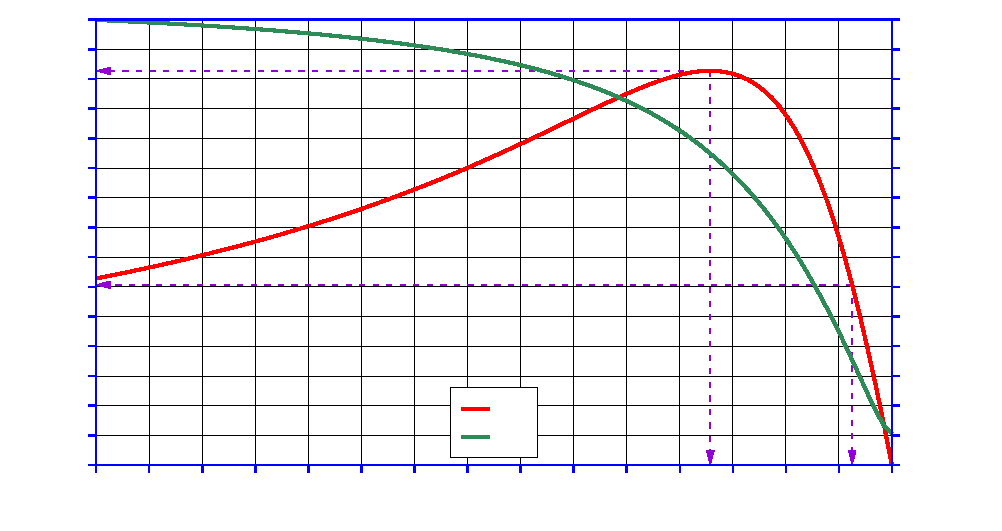
\includegraphics{Cap-Motors-Induccio-Ex4}}%
    \gplfronttext
  \end{picture}%
\endgroup

    \end{center}

\end{exemple}

\section{Norma NEMA MG-1}\index{NEMA!MG-1}

La «National Electrical Manufacturers Association» (NEMA),
tracta en la norma  MG-1 «Motors and Generators» una gran quantitat de qüestions de tota mena relatives a motors i generadors, tant trifàsics com monofàsics, de corrent continu i de corrent altern.

S'expliquen a continuació algunes de les qüestions d'aquesta norma que són d'aplicació als motors d'inducció trifàsics.

\subsection{Punts característics de la corba parell--velocitat}
\index{NEMA!MG-1!punts característics en la corba parell--velocitat}

En la Figura \vref{pic:mot-punts-T-vel} es representa una corba típica parell--velocitat d'un motor, assenyalant-hi quatre punts als quals la norma NEMA MG-1 els dona uns noms característics. En l'eix d'abscisses s'hi pot representar indistintament les velocitats de rotació $\omega\ped{m}$ o $n\ped{m}$, o  el lliscament $s$ (amb valors que van des d'1, arrencada, fins a 0, velocitat síncrona $\omega\ped{m,sinc}$).
\begin{center}
    \input{Imatges/Cap-Motors-Induccio-Punts-T-vel.pdf_tex}
    \captionof{figure}{Punts característics d'una corba parell--velocitat}
    \label{pic:mot-punts-T-vel}
\end{center}

Es dona a continuació la definició dels quatre punts de la Figura  \vref{pic:mot-punts-T-vel}.

\begin{dingautolist}{'312}
   \item «Locked-rotor torque» (parell d'arrencada). També s'anomena «starting torque», «stall torque» o «breakaway torque». És el mínim parell $T\ped{m,arr}$ que es produeix amb el motor aturat, per a qualsevol posició angular del rotor, quan s'aplica al motor la tensió nominal a la freqüència nominal.
   \item «Pull-up torque» (parell mínim). És el mínim parell $T\ped{m,\text{mín}}$ que es produeix durant el període d'acceleració del motor, entre l'arrancada  i el parell màxim $T\ped{m,\text{màx}}$. En el cas dels motors que no tenen un parell màxim definit, el «pull-up torque» és el mínim parell que es produeix fins arribar a la velocitat nominal $\omega\ped{m,N}$.
   \item «Breakdown torque» (parell màxim). També s'anomena «pull-out torque». És el màxim parell $T\ped{m,\text{màx}}$ que  produeix  el motor, quan se li aplica  la tensió nominal a la freqüència nominal, sense cap variació abrupta de la velocitat.
   \item «Full load torque» (parell nominal). És el parell necessari $T\ped{m,N}$ per produir la potència mecànica nominal del motor a la velocitat nominal  $\omega\ped{m,N}$.
\end{dingautolist}
\index{parell!d'arrencada}\index{parell!mínim}\index{parell!màxim}\index{parell!nominal}
\index{locked@«locked-rotor torque»}\index{pullup@«pull-up torque»}\index{breackdown@«breakdown torque»}\index{full@«full load torque»}\index{pullout@«pull-out torque»}\index{starting@«starting torque»}\index{breakaway@«breakaway torque»}\index{stall@«stall torque»}


\subsection{Codi de lletres de corrent d'arrencada}
\index{NEMA!MG-1!codi de lletres de corrent d'arrencada}

El corrent d'arrencada d'un motor pot indicar-se directament en ampere, o com un múltiple del corrent nominal (per exemple: $I\ped{arr} = 6 I\ped{N}$). No obstant, els motors que segueixen la NEMA MG-1, també poden indicar aquest corrent mitjançant d'una lletra, anomenada «code letter for locked-rotor kVA». A cada lletra li correspon un valor (de fet un rang de valors possibles) que dona la relació entre la potencia elèctrica aparent absorbida pel motor en el moment d'arrencar, expressada en kVA, i la potència mecànica nominal del motor, expressada en HP, quan el motor s'alimenta a la tensió nominal; si anomenem $\kappa$ a aquesta relació, tenim:
\begin{equation}
    \kappa = \frac{S\ped{arr}/{\scriptstyle\si{kVA}}}{P\ped{m,N}/{\scriptstyle \si{HP}}}
\end{equation}

Expressem a continuació la potencia elèctrica aparent, en kVA, absorbida pel motor en el moment d'arrencar, a partir de la tensió nominal d'alimentació i del corrent d'arrencada:
\begin{equation}
    S\ped{arr}/{\scriptstyle \si{kVA}} = \frac{\sqrt{3}\,U\ped{N}/{\scriptstyle \si{V}}\,I\ped{arr}/{\scriptstyle \si{A}}}{1000}
\end{equation}

A partir de les dues equacions anteriors, podem obtenir el valor del corrent d'arrencada:
\begin{equation}
    I\ped{arr}/{\scriptstyle \si{A}} = \frac{1000 \,\kappa}{\sqrt{3}} \,\frac{P\ped{m,N}/{\scriptstyle \si{HP}}}{U\ped{N}/{\scriptstyle \si{V}}} = \num{577,35}\,\kappa\,\frac{P\ped{m,N}/{\scriptstyle \si{HP}}}{U\ped{N}/{\scriptstyle \si{V}}}\label{eq:LR-code}
\end{equation}

En la Taula \vref{taula:LR-code} es dona el rang de valors que pren $\kappa$ per a cadascuna de les lletres d'aquest codi. El valor superior de cada rang en queda exclòs.

\begin{longtable}[h]{cc}
   \caption{\label{taula:LR-code} «Code letters for locked-rotor kVA»}\\
   \toprule[1pt]
    Lletra NEMA & Rang de valors de $\kappa$\\
   \midrule
   \endfirsthead
   \caption[]{«Code letters for locked-rotor kVA» (\emph{ve de la pàgina anterior})}\\
   \toprule[1pt]
    Lletra NEMA & Rang de valors de $\kappa$\\
   \midrule
   \endhead
   \midrule
   \multicolumn{2}{r}{\sffamily\bfseries\color{NavyBlue}(\emph{continua a la pàgina següent})}
   \endfoot
   \endlastfoot
    A & \numrange{0,00}{3,15} \\
    B & \numrange{3,15}{3,55} \\
    C & \numrange{3,55}{4,0} \\
    D & \numrange{4,0}{4,5} \\
    E & \numrange{4,5}{5,0} \\
    F & \numrange{5,0}{5,6} \\
    G & \numrange{5,6}{6,3} \\
    H & \numrange{6,3}{7,1} \\
    J & \numrange{7,1}{8,0}\\
    K & \numrange{8,0}{9,0} \\
    L & \numrange{9,0}{10,0} \\
    M & \numrange{10,0}{11,2} \\
    N & \numrange{11,2}{12,5} \\
    P & \numrange{12,5}{14,0} \\
    R & \numrange{14,0}{16,0} \\
    S & \numrange{16,0}{18,0} \\
    T & \numrange{18,0}{20,0} \\
    U & \numrange{20,0}{22,4} \\
    V & \num{22,4} i superior \\
\bottomrule[1pt]
\end{longtable}
\index{A} \index{B} \index{C} \index{D}\index{E} \index{F} \index{G} \index{H}\index{J} \index{K} \index{L} \index{M}\index{N} \index{P} \index{R} \index{S}\index{T} \index{U} \index{V}

\addcontentsxms{Corrent d'arrenca  d'un motor segons NEMA MG-1}
\begin{exemple}[Corrent d'arrenca  d'un motor segons NEMA MG-1]
    Sabent que la  potència nominal d'un motor és: $P\ped{m,N} = \SI{7,5}{HP}$,    que la seva tensió nominal és: $U\ped{N}=\SI{400}{V}$, i que la lletra NEMA és: H, es tracta de trobar el corrent d'arrencada  del  motor i el seu valor en relació al corrent nominal.

    Si prenem per a la lletra H el valor mitjà del seu rang: $\kappa = \frac{\num{6,3}+\num{7,1}}{2}=\num{6,7}$, a partir de l'equació  \eqref{eq:LR-code} tenim:
    \[
      I\ped{arr} = \num{577,35} \times \num{6,7} \times \frac{\SI{7,5}{HP}}{\SI{400}{V}} = \SI{72,5}{A}
    \]

    Donat que no tenim cap dada sobre el corrent nominal, calcularem primer la potència aparent nominal de forma aproximada utilitzant l'equació \eqref{eq:kVA-CV-HP}:
    \[
        S\ped{N} \approx \SI{7,5}{kVA}
    \]

    Calculem ara el corrent nominal:
    \[
        I\ped{N}= \frac{S\ped{N}}{\sqrt{3} U\ped{N}} = \frac{\SI{7500}{VA}}{\sqrt{3}\times\SI{400}{V}} = \SI{10,8}{A}
    \]

    La relació entre el corrent d'arrencada i el corrent nominal és doncs:
    \[
        \frac{I\ped{arr}}{I\ped{N}} = \frac{\SI{72,5}{A}}{\SI{10,8}{A}} = \num{6,7}
    \]

    Com es pot veure, el valor  de $\kappa$ de la taula \vref{taula:LR-code} és aproximadament igual al valor de $I\ped{arr}/I\ped{N}$.

    Aquesta igualtat entre $I\ped{arr}/I\ped{N}$ i $\kappa$ només es dona quan l'equació \eqref{eq:kVA-CV-HP} és vàlida, és a dir quan es compleix $S\ped{N}/{\scriptstyle \si{kVA}} \approx  P\ped{m,N}/{\scriptstyle \si{HP}}$.

    En canvi, en el cas, per exemple, d'un motor amb les característiques: $P\ped{m,N} = \SI{0,54}{HP}$, $U\ped{N} = \SI{380}{V}$, $I\ped{N} = \SI{1,4}{A}$, $I\ped{arr} = \SI{8,2}{A}$ i lletra NEMA L, veiem que el valor de \SI{8,2}{A} és el que correspon a prendre  el valor màxim $\kappa = 10$ de la lletra L:
    \[
      I\ped{arr} = \num{577,35} \times 10 \times \frac{\SI{0,54}{HP}}{\SI{380}{V}} = \SI{8,2}{A}
    \]

    Però la relació entre el corrent d'arrencada i el corrent nominal és:
    \[
        \frac{I\ped{arr}}{I\ped{N}} = \frac{\SI{8,2}{A}}{\SI{1,4}{A}} = \num{5,9}
    \]

    I per tant  en aquest cas tenim $\kappa \neq I\ped{arr}/I\ped{N}$, la qual cosa ens indica que l'equació \eqref{eq:kVA-CV-HP} no és aplicable en aquest cas.
\end{exemple}

\subsection{Tensions desequilibrades}
\index{NEMA!MG-1!tensions desequilibrades}

Un motor consumeix el corrent nominal quan subministra la potència mecànica nominal girant a la velocitat nominal, i està alimentat a la tensió nominal. Per tal que això sigui cert, la tensió d'alimentació trifàsica ha de ser equilibrada.

Quan la tensió trifàsica d'alimentació és desequilibrada, el corrent necessari per subministrar la potència mecànica nominal, és més gran que el corrent nominal. A més, un desequilibri de tensions relativament petit, produeix un increment del corrent proporcionalment molt gran, generant un  calor addicional que el motor haurà d'evacuar, i una possible actuació de les proteccions elèctriques del motor.

En aquestes condicions de tensió desequilibrada, cal reduir el valor de la potència mecànica nominal del motor per tal que el corrent baixi al seu valor nominal.

La norma NEMA MG-1 proporciona una gràfica que dona un factor reductor de la potència mecànica nominal, que anomenarem $\kappa\ped{P}$, en funció de desequilibris de tensions de fins el \SI{5}{\%}. El desequilibri de tensions $\Deltaup u$ el defineix com:
\[
    \Deltaup u = \frac{\text{màxima desviació de la tensió respecte del valor mitja}}{\text{valor mitjà de la tensió}}
\]

En la Figura \vref{pic:Du-kp-ki} es representa aquest factor reductor $\kappa\ped{P}$ en funció de $\Deltaup u$.

Si tenim en compte que  $\kappa\ped{P}$ és el valor pel qual cal multiplicar la potència mecànica nominal per fer baixar el corrent fins el seu valor nominal, i que la potència és proporcional al corrent, podem deduir que si es volgués mantenir la potència nominal mecànica, el corrent augmentaria en un factor, que anomenarem $\kappa\ped{I}$, que variaria de forma inversa a $\kappa\ped{P}$: $\kappa\ped{I}=\frac{1}{\kappa\ped{P}}$. En la Figura \vref{pic:Du-kp-ki} es representa també aquest factor $\kappa\ped{I}$ en funció de la mateixa $\Deltaup u$.

Com es pot veure, si el desequilibri de tensions arribés al \SI{5}{\%}, caldria reduir la potència nominal mecànica del motor, multiplicant-la pel factor  $\kappa\ped{P}= \num{0,755}$, ja que si no es fes el corrent augmentaria en
un factor $\kappa\ped{I}= \num{1,325}$.

\begin{center}
    % GNUPLOT: LaTeX picture with Postscript
\begingroup
  \makeatletter
  \providecommand\color[2][]{%
    \GenericError{(gnuplot) \space\space\space\@spaces}{%
      Package color not loaded in conjunction with
      terminal option `colourtext'%
    }{See the gnuplot documentation for explanation.%
    }{Either use 'blacktext' in gnuplot or load the package
      color.sty in LaTeX.}%
    \renewcommand\color[2][]{}%
  }%
  \providecommand\includegraphics[2][]{%
    \GenericError{(gnuplot) \space\space\space\@spaces}{%
      Package graphicx or graphics not loaded%
    }{See the gnuplot documentation for explanation.%
    }{The gnuplot epslatex terminal needs graphicx.sty or graphics.sty.}%
    \renewcommand\includegraphics[2][]{}%
  }%
  \providecommand\rotatebox[2]{#2}%
  \@ifundefined{ifGPcolor}{%
    \newif\ifGPcolor
    \GPcolortrue
  }{}%
  \@ifundefined{ifGPblacktext}{%
    \newif\ifGPblacktext
    \GPblacktexttrue
  }{}%
  % define a \g@addto@macro without @ in the name:
  \let\gplgaddtomacro\g@addto@macro
  % define empty templates for all commands taking text:
  \gdef\gplbacktext{}%
  \gdef\gplfronttext{}%
  \makeatother
  \ifGPblacktext
    % no textcolor at all
    \def\colorrgb#1{}%
    \def\colorgray#1{}%
  \else
    % gray or color?
    \ifGPcolor
      \def\colorrgb#1{\color[rgb]{#1}}%
      \def\colorgray#1{\color[gray]{#1}}%
      \expandafter\def\csname LTw\endcsname{\color{white}}%
      \expandafter\def\csname LTb\endcsname{\color{black}}%
      \expandafter\def\csname LTa\endcsname{\color{black}}%
      \expandafter\def\csname LT0\endcsname{\color[rgb]{1,0,0}}%
      \expandafter\def\csname LT1\endcsname{\color[rgb]{0,1,0}}%
      \expandafter\def\csname LT2\endcsname{\color[rgb]{0,0,1}}%
      \expandafter\def\csname LT3\endcsname{\color[rgb]{1,0,1}}%
      \expandafter\def\csname LT4\endcsname{\color[rgb]{0,1,1}}%
      \expandafter\def\csname LT5\endcsname{\color[rgb]{1,1,0}}%
      \expandafter\def\csname LT6\endcsname{\color[rgb]{0,0,0}}%
      \expandafter\def\csname LT7\endcsname{\color[rgb]{1,0.3,0}}%
      \expandafter\def\csname LT8\endcsname{\color[rgb]{0.5,0.5,0.5}}%
    \else
      % gray
      \def\colorrgb#1{\color{black}}%
      \def\colorgray#1{\color[gray]{#1}}%
      \expandafter\def\csname LTw\endcsname{\color{white}}%
      \expandafter\def\csname LTb\endcsname{\color{black}}%
      \expandafter\def\csname LTa\endcsname{\color{black}}%
      \expandafter\def\csname LT0\endcsname{\color{black}}%
      \expandafter\def\csname LT1\endcsname{\color{black}}%
      \expandafter\def\csname LT2\endcsname{\color{black}}%
      \expandafter\def\csname LT3\endcsname{\color{black}}%
      \expandafter\def\csname LT4\endcsname{\color{black}}%
      \expandafter\def\csname LT5\endcsname{\color{black}}%
      \expandafter\def\csname LT6\endcsname{\color{black}}%
      \expandafter\def\csname LT7\endcsname{\color{black}}%
      \expandafter\def\csname LT8\endcsname{\color{black}}%
    \fi
  \fi
    \setlength{\unitlength}{0.0500bp}%
    \ifx\gptboxheight\undefined%
      \newlength{\gptboxheight}%
      \newlength{\gptboxwidth}%
      \newsavebox{\gptboxtext}%
    \fi%
    \setlength{\fboxrule}{0.5pt}%
    \setlength{\fboxsep}{1pt}%
\begin{picture}(9340.00,5100.00)%
    \gplgaddtomacro\gplbacktext{%
      \colorrgb{0.00,0.00,0.00}%%
      \put(921,787){\makebox(0,0)[r]{\strut{} 0,70}}%
      \colorrgb{0.00,0.00,0.00}%%
      \put(921,1469){\makebox(0,0)[r]{\strut{} 0,75}}%
      \colorrgb{0.00,0.00,0.00}%%
      \put(921,2151){\makebox(0,0)[r]{\strut{} 0,80}}%
      \colorrgb{0.00,0.00,0.00}%%
      \put(921,2834){\makebox(0,0)[r]{\strut{} 0,85}}%
      \colorrgb{0.00,0.00,0.00}%%
      \put(921,3516){\makebox(0,0)[r]{\strut{} 0,90}}%
      \colorrgb{0.00,0.00,0.00}%%
      \put(921,4198){\makebox(0,0)[r]{\strut{} 0,95}}%
      \colorrgb{0.00,0.00,0.00}%%
      \put(921,4880){\makebox(0,0)[r]{\strut{} 1,00}}%
      \colorrgb{0.00,0.00,0.00}%%
      \put(1105,481){\makebox(0,0){\strut{} 0,0}}%
      \colorrgb{0.00,0.00,0.00}%%
      \put(1870,481){\makebox(0,0){\strut{} 0,5}}%
      \colorrgb{0.00,0.00,0.00}%%
      \put(2635,481){\makebox(0,0){\strut{} 1,0}}%
      \colorrgb{0.00,0.00,0.00}%%
      \put(3401,481){\makebox(0,0){\strut{} 1,5}}%
      \colorrgb{0.00,0.00,0.00}%%
      \put(4166,481){\makebox(0,0){\strut{} 2,0}}%
      \colorrgb{0.00,0.00,0.00}%%
      \put(4931,481){\makebox(0,0){\strut{} 2,5}}%
      \colorrgb{0.00,0.00,0.00}%%
      \put(5696,481){\makebox(0,0){\strut{} 3,0}}%
      \colorrgb{0.00,0.00,0.00}%%
      \put(6461,481){\makebox(0,0){\strut{} 3,5}}%
      \colorrgb{0.00,0.00,0.00}%%
      \put(7227,481){\makebox(0,0){\strut{} 4,0}}%
      \colorrgb{0.00,0.00,0.00}%%
      \put(7992,481){\makebox(0,0){\strut{} 4,5}}%
      \colorrgb{0.00,0.00,0.00}%%
      \put(8757,481){\makebox(0,0){\strut{} 5,0}}%
    }%
    \gplgaddtomacro\gplfronttext{%
      \csname LTb\endcsname%%
      \put(291,2833){\makebox(0,0){\strut{}$\kappa\ped{P}$}}%
      \csname LTb\endcsname%%
      \put(8902,2833){\makebox(0,0){\strut{}}}%
      \csname LTb\endcsname%%
      \put(4931,153){\makebox(0,0){\strut{}$\Deltaup u\, / \,\unit{\%}$}}%
      \csname LTb\endcsname%%
      \put(4931,4771){\makebox(0,0){\strut{}}}%
      \csname LTb\endcsname%%
      \put(4931,4880){\makebox(0,0){\strut{}}}%
    }%
    \gplbacktext
    \put(0,0){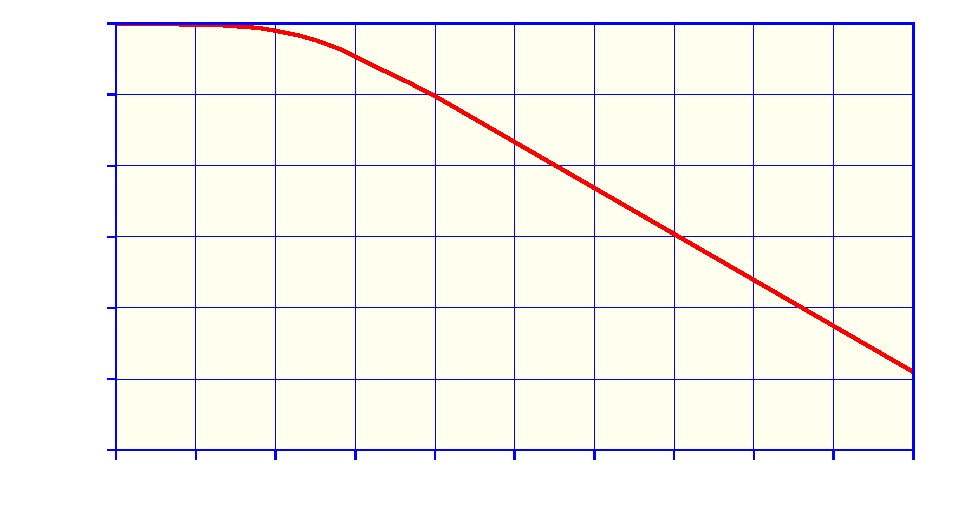
\includegraphics{Cap-Motors-Induccio-U-Deseq}}%
    \gplfronttext
  \end{picture}%
\endgroup

    \captionof{figure}{Tensió d'alimentació desequilibrada en motors}
    \label{pic:Du-kp-ki}
\end{center}

\addcontentsxms{Tensió d'alimentació desequilibrada en un motor}
\begin{exemple}[Tensió d'alimentació desequilibrada en un motor]
    Sabent que la  potència nominal d'un motor és: $P\ped{m,N} = \SI{7,5}{HP}$, i que les tres tensions desequilibrades  de fase tenen els valors: 460 V, 467 V i 450 V, es tracta de trobar els factor $\kappa\ped{P}$ i  $\kappa\ped{I}$, i el valor de la potència nominal corregida.

    Calculem primer el valor mitjà de la tensió:
    \[
      \bar{U} = \frac{\SI{460}{V}+\SI{467}{V}+\SI{450}{V}}{3} = \SI{459}{V}
    \]

    La màxima desviació de les tres tensions respecte d'aquest valor és: $\SI{459}{V}-\SI{450}{V} = \SI{9}{V}$. Per tant tenim:
    \[
        \Deltaup u = \frac{\SI{9}{V}}{\SI{459}{V}} = \num{1,96e-2} = \SI{1,96}{\%}
    \]

     A partir d'aquest valor, trobem a la Figura \vref{pic:Du-kp-ki} els valors:  $\kappa\ped{P} = \num{0,95}$ i  $\kappa\ped{I}=\num{1,05}$.

     Per tant, per tal que el corrent no augmenti en un factor de 1,05, haurem de reduir la potència nominal a:
     \[
         P'\ped{m,N} = \num{0,95}\times{}P\ped{m,N}  = \num{0,95}\times\SI{7,5}{HP} = \SI{7,1}{HP}
     \]
\end{exemple}

\subsection{Classes d'aïllaments tèrmics en motors}
\index{NEMA!MG-1!classes d'a\"{i}llaments tèrmics}

Quan es posa en marxa un motor, la seva temperatura comença a pujar
per sobre de la temperatura ambient a causa del corrent que circula
pels seus debanats.

La norma NEMA MG-1 defineix diverses classes d'aïllament tèrmic, depenent de
l'increment global de temperatura permès respecte de la temperatura
ambient, que fixa en \SI{40}{\degreeCelsius};\index{temperatura!ambient}
per a cada classe es permet un increment addicional de temperatura
en el punt més calent, situat en el centre dels debanats del
motor.\index{temperatura!en el punt més calent}

En la Taula \vref{taula:classes-nema} es donen els valors dels increments de temperatura permesos per a cadascuna de les diferents classes d'aïllament, partint d'una temperatura ambient de \SI{40}{\degreeCelsius}.

\begin{center}
   \captionof{table}{Classes NEMA d'aïllaments tèrmics en motors} \label{taula:classes-nema}
   \begin{tabular}{cr<{\hspace{6em}}r<{\hspace{8em}}}
   \toprule[1pt]
   Classe & \multicolumn{1}{c}{Increment global de temperatura} & \multicolumn{1}{c}{Increment addicional de temperatura} \\
   NEMA &   \multicolumn{1}{c}{sobre la temperatura ambient}  & \multicolumn{1}{c}{en el punt més calent} \\
   \midrule
   A & \SI{60}{\degreeCelsius} & \SI{5}{\degreeCelsius}   \\
   B & \SI{80}{\degreeCelsius} & \SI{10}{\degreeCelsius}   \\
   F & \SI{105}{\degreeCelsius} & \SI{10}{\degreeCelsius}   \\
   H & \SI{125}{\degreeCelsius} & \SI{15}{\degreeCelsius}   \\
   \bottomrule[1pt]
   \end{tabular}
\end{center}
\index{A} \index{B} \index{F} \index{H}

